\documentclass[12pt]{article}
\usepackage[
left=2.50cm,
right=2.50cm,
top=2.50cm,
bottom=2.50cm
]{geometry}
\geometry{a4paper}
\usepackage[T1]{fontenc}
\usepackage[utf8]{inputenc}
\usepackage{authblk}
%\usepackage[backend=biber]{biblatex}
%\addbibresource{biblio.bib}
\usepackage[running]{lineno}
\usepackage[round]{natbib}
\usepackage{graphicx}
\usepackage{setspace}
\usepackage{amsmath}
\usepackage{amssymb}
\usepackage{pdfpages}
\usepackage[
colorlinks,
citecolor=blue,
urlcolor=cyan,
bookmarks=true,
hypertexnames=true
]{hyperref}
%\onehalfspacing
\newcommand{\I}{\mathbb{I}}
\renewcommand\refname{\textsc{Literature Cited}}

\usepackage{sectsty}
\sectionfont{\centering}
\subsectionfont{\centering}
\subsubsectionfont{\centering}

\title{\textbf{{\Huge Long-term demographic dynamics of a keystone scavenger disrupted by human-induced shifts in food availability}}}

\author[a]{Pablo Almaraz\thanks{\textit{E-mail address}: pablo.almaraz@csic.es (Pablo Almaraz),  Phone: +34 956 832 612 Ext. 255}}
\author[b]{Félix Martínez}
\author[c]{Zebensui Morales-Reyes}
\author[c]{José A. Sánchez-Zapata}
\author[d]{Guillermo Blanco}

\affil[a]{Department of Ecology and Coastal Management, Instituto de Ciencias Marinas de Andalucía, ICMAN-CSIC, Campus Río San Pedro, 11510, Puerto Real, Spain.}
\affil[b]{Escuela Internacional de Doctorado, Universidad Rey Juan Carlos (URJC), C/ Tulipán s/n, E-28933 Móstoles, Madrid, Spain. }
\affil[c]{Departamento de Biología Aplicada, Universidad Miguel Hernández, Avda. de la Universidad, s/n, 03202 Elche, Alicante, Spain.}
\affil[d]{Department of Evolutionary Ecology, Museo Nacional de Ciencias Naturales (MNCN-CSIC), José Gutiérrez Abascal 2, 28006 Madrid, Spain.}

%\renewcommand\Authands{ and }
\renewcommand\Authands{,}

%\date{\today}
\date{\textbf{Open Research statement}: The code for the model described in the paper is included as DataS1. All data, code, and scripts needed for reproducing the results presented here is archived in Dryad, Zenodo  and GitHub \url{https://github.com/palmaraz/SaniVult}.\\

\vspace{1in}

\textbf{Running Head}: Keystone scavengers and sanitary policy}

\begin{document}

\maketitle

\newpage

\doublespacing

% Running head: Keystone species and sanitary regulation

%\section*{\textit{Abstract}}
\linenumbers
%\noindent\rule{\textwidth}{1pt}
\textit{Abstract.} \quad Scavenging is a key ecological process controlling energy flow in ecosystems and providing valuable ecosystem services worldwide. As long-lived species, the demographic dynamics of vultures can be disrupted by spatio-temporal fluctuations in food availability, with dramatic impacts on their population viability and the ecosystem services provided. In Europe, the outbreak of Bovine Spongiform Encephalopathy (BSE) in 2001 prompted a restrictive sanitary legislation banning the presence of livestock carcasses in the wild at a continental scale. In long-lived vertebrate species the buffering hypothesis predicts that the demographic traits with the largest contribution to population growth rate should be less temporally variable. The BSE outbreak provides a unique opportunity to test for the impact of demographic buffering in a keystone scavenger suffering abrupt but transient food shortages. We study the 42-year dynamics (1978-2020) of one of the world’s largest breeding colonies of Eurasian griffon vultures (\textit{Gyps fulvus}). We fitted an inverse Bayesian state-space model with density-dependent demographic rates to the time-series of stage-structured abundances to investigate shifts in vital rates and population dynamics before, during and after the implementation of a restrictive sanitary regulation. Prior to the BSE outbreak the dynamics was mainly driven by adult survival: 83\% of temporal variance in abundance was explained by variability in this rate. Moreover, during this period the regulation of population size operated through density-dependent fecundity and sub-adult survival. However, after the onset of the European ban, a one-month delay in average laying date, a drop in fecundity and a reduction in the number of fledglings induced a transient increase in the impact of fledgling and sub-adult recruitment on dynamics. Although adult survival rate remained constantly high, as predicted by the buffering hypothesis, its relative impact on the temporal variance in abundance dropped to 71\% during the sanitary legislation and to 54\% after the ban was lifted. A significant increase in the relative impact of environmental stochasticity on dynamics was modeled after the BSE outbreak. These results provide empirical evidence on how abrupt environmental deterioration may induce dramatic demographic and dynamic changes in the populations of keystone scavengers, with far-reaching impacts on ecosystem functioning worldwide.

%\section*{\textit{Key words}}
%\noindent\rule{\textwidth}{1pt}
\textit{Key words}:  \textit{carrion; inverse demographic modelling; mad cow disease; matrix modelling; state-space modelling; scavenging; vultures.}
%\newpage

\vspace*{0.5in}

\section*{\textsc{Introduction}}

Predictable food subsidies from humans are increasingly altering ecosystem structure and functioning in multiple ways, with far-reaching consequences for environmental conservation worldwide (\cite{Oro2013}). Such food subsidies are known to influence the population size and trends of different generalist vertebrate species. For example, seabirds usually benefit from fisheries discards (e.g., \cite{Bicknell2013}), garden birds from supplementary feeding in urban areas (e.g. \cite{Fuller2008}) or game species including mammals and birds from diversionary and management feeding (e.g. \cite{Putman2004}). Scavengers are among these vertebrates that are tightly linked to food subsidies derived from human activities including shepherding, hunting and supplementary feeding (\cite{Donazar1993,Mateo-Tomas2010b,Blanco2014,Cortes-Avizanda2016}). Interactions between humans and scavengers have been closely connected since the Late Pliocene when early hominids probably competed for food with other scavengers (\cite{Moleon2014}). Nowadays, even if wild ungulate carcasses from hunting are an important source of food for scavengers, these species mostly rely on livestock for food worldwide (\cite{Donazar1993,Mateo-Tomas2015,Lambertucci2009,Lambertucci2018}). Indeed, beyond the ecological function of eliminating wild ungulate carcasses, vertebrate scavengers provide an important ecosystem service by eliminating both domestic ungulate carcasses from agricultural waste, and carcasses derived from hunting (\cite{Moleon2014a,Morales-Reyes2015,DeVault2016})\\

Among vertebrates, vultures are one of the most threatened scavengers worldwide (\cite{Buechley2016}). The main extrinsic threats for vultures include dietary pollutants (i.e. poisoning and veterinary drugs such as diclofenac and antibiotics), collision and electrocution with electric infrastructures, direct persecution and reduction in food availability (\cite{Ogada2012,Blanco2016,Buechley2016}). Carcass availability might be subject to changes related to socioeconomic shifts in livestock production and management (e.g. the abandonment of traditional farming practices; \cite{Olea2009}), rewilding processes (e.g. increase of wild ungulate populations; \cite{Cortes-Avizanda2015}) or sanitary regulations (\cite{Margalida2010,Blanco2014}). Thus, these changes might affect not only resource availability but also their predictability and quality (\cite{Donazar2009b,Cortes-Avizanda2012,Blanco2014,Blanco2017,Blanco2019}). These factors can have a profound influence on population dynamics by driving key demographic parameters ultimately determining population dynamics, age structure and reproductive performance. The life-history strategies of long-lived species in fluctuating environments are predicted to evolve to reduce the temporal variability of population growth rate (\cite{Roff2002,Doak2005}). In particular, the demographic buffering hypothesis (\cite{Pfister2002}) predicts that those demographic rates with a larger contribution to growth rate, and hence with a larger impact on extinction probability, should be less variable across time. Since population growth rate is particularly sensitive to adult survival in long-lived species (\cite{Saether2000,Gaillard2010}), canalized adult survival is predicted to stabilize long term dynamics (e.g., \cite{Rotella2019}). In unpredictable environments, in particular in the presence of abrupt perturbations on demographic rates induced by human activities, the ability of populations of long-lived species to buffer those rates more strongly affecting population growth will determine their extinction probability. Nevertheless, there is little evidence on the magnitude of the effects of changes in food availability on the long-term demography and population dynamics of long-lived scavenger species (\cite{Margalida2014b}). \\

In Europe, the outbreak of Bovine Spongiform Encephalopathy (BSE) led to the subsequent application of a restrictive sanitary legislation that critically limited the use of animal by-products not intended for human consumption (Regulation EC 1774/2002). This legislation banned the disposal of livestock carcasses in the field, which originated a major conservation problem, namely a new source of greenhouse gases emissions associated with the destruction of carcasses in authorized plants (\cite{Morales-Reyes2015}), and further affected the ecosystem services provided by scavengers (\cite{Margalida2012,Blanco2014,Moleon2014a,Morales-Reyes2015}). This conflict between sanitary and environmental policies led to an intense debate about the European dispositions that regulated the use of animal by-products and their implications for conservation of necrophagous birds (\cite{Tella2001,Donazar2009b,Margalida2010}). In particular, virtual population modelling predicts that food shortage derived from sanitary regulations may induce rapid population declines in the Eurasian griffon vulture (\textit{Gyps fulvus}) (\cite{Margalida2012}). This colonial species is by far the most abundant and widespread obligate scavenger in Europe, and is also considered the dominant species in scavenger guilds (\cite{Cortes-Avizanda2012}). Roughly, 30000-37000 pairs currently breed in Spain (> 95\% of the EU population (\cite{Moral2018}). However, there is a lack of knowledge on the long-term breeding biology and on the demographic consequences of sanitary regulation on vultures’ population dynamics and conservation.\\

Here, we take advantage of the long-term monitoring of one of the largest colonies of Eurasian griffon vultures in Europe to analyse multi-decadal changes in the demographic dynamics of this species. The different trophic scenarios that arose after the dramatic change in food availability derived from the European sanitary regulations provides an excellent opportunity to conduct a natural experiment to study aspects of demography and population dynamics directly dependent on food availability that can be hardly reproduced experimentally. The main goal of this analysis will be to model the long-term dynamics of vital rates before, during and after the implementation of the European sanitary regulation EC 1774/2002, in order to explore potential temporal shifts in the demographic structure induced by abrupt environmental deterioration. According to the buffering hypothesis (\cite{Pfister2002}) we predict that adult survival of vultures remained constant in spite of the abrupt food shortage. In particular, within this scenario we evaluated how a large shift in food availability derived from the application of sanitary regulations affected, i) the population size, ii) stage structure, iii) laying dates and iv) breeding success of Eurasian griffon vultures, and how these traits impacted upon long-term population dynamics.

\section*{\textsc{Materials and methods}}

\subsection*{\textit{Study area and fieldwork}}
We collected demographic data in the gorges of the Riaza River (41º31'N, 3º36'W), north of Segovia Province, Central Spain. The area includes a complex of cliffs and canyons where a large population of about 720 pairs of Eurasian griffon vulture breeds. We censused the colony every two or three years from 1984 to 1994 and then annually until 2020; further information was obtained from the national census of 1979 and other sources (\url{http://www.naturalicante.com/mochila/Montejo/Hojas-e-Informes-censo.htm}). We conducted five complete surveys each breeding season in order to detect all pairs (\cite{Martinez1997}). We examined both partners of each breeding pair to assess whether they were morphologically adults or sub-adults; individuals were categorized as sub-adults when they had not acquired full adult appearance (at 5-6 years old) on the basis of their general body colour, bill colour and, especially the colour, length and shape of the ruff feathers (\cite{Elosegui1989,Blanco1996,Duriez2011}). The age structure of pairs was recorded in three possible combinations: adult-adult, adult-sub-adult and sub-adult-sub-adult (\cite{Blanco1996,Blanco1997}). To control for errors in the stage-classification of the monitored individuals due to uncertain ageing, we specified a state-space approach (\cite{King2010}) linking the demographic process to the data through an observation model (see subsection \textbf{Observation model}).\\

Breeding Eurasian griffon vultures are year-round residents in the study area. Egg laying began in late December and the last clutches were laid by mid-March (\cite{Martinez1998}). We conducted regular and intensive monitoring throughout the breeding season to determine whether the pairs laid (breeding pairs) or do not laid (non-breeding pairs) despite they showed typical pair-bonding behavior, including close contact, nest building and defense, and copulation. We observed at a distance the presence of eggs in the nests, recorded the start of incubation and calculated the date of hatching based on nestling age (\cite{Elosegui1989}). Taking into account all these criteria and an incubation period of 55 days we determined laying dates within 10-day periods from 10 December onward (\cite{Martinez1998}). Nests were regularly checked to verify breeding failure or the success of each pair in fledgling young; young fledged from June-August (\cite{Fargallo2018}). All observations were made by telescope at distances that avoided disturbing the birds in the colony. Besides the long-term monitoring of breeding pairs in the colony, we focused on the behavior of 456 individuals ringed as nestlings since 1990. Of these individuals, only 9 bred outside the focal colony and most in colonies <50 Kms. away from there. In contrast, 136 birds bred or attempted to bred in the focal colony, some for more than 20 years. These data point to the strong philopatry of the Eurasian griffon vulture to the study area (F. Martínez and G. Blanco in prep.). These results agree with the dispersal behavior of the studied species in other colonies (\cite{Zuberogoitia2013}). Overall, we considered breeders in this population as highly philopatric to their natal colony


\subsection*{\textit{Stage-structured density-dependent population dynamics model}}

Demographic population modelling is usually conducted through the use of population projection matrices (\cite{Caswell2001}). This direct approach uses empirical estimates of vital rates, such as age-dependent fecundity and survival, to project the rate of increase of a population. In the presence of age- or stage-structured population time series, an alternative approach is to use inverse demographic modelling (\cite{Wood1997,Caswell2001}). In this approach, vital rates are estimated through the fitting of a set of difference equations describing the life-history of a species to age- or stage-structured time series data (\cite{Wood1994,Caswell2001,Gross2002,Wielgus2008}). In this study, we fit an inverse Bayesian stage-structured stochastic density-dependent demographic model to data assembled from distance observations of multiple cohorts of individuals during a 42-year period. As a non-invasive demographic approach (\cite{Wielgus2008}), this method allows for the estimation of demographic vital rates from population-abundance data, with no need of capturing-recapturing individuals across time. Although this approach has been used previously (\cite{Gross2002,Wielgus2008}), these implementations were deterministic. In contrast, here we propose a fully stochastic strategy taking into account demographic and environmental stochasticity, as well as sampling error and missing data. Our Bayesian approach thus allows for the efficient propagation and classification of uncertainty from the data to vital rates and population growth rates.\\

The demographic model for the Eurasian griffon vulture is based on the standard avian life cycle (\cite{Bennett2002}). This model considers three separate demographic stages: fledglings, sub-adults and adults (Appendix S1: Fig. S1). Three transitions among life stages and two survival probabilities define the time-relationships between stages, so a set of three difference equations, including environmental and demographic stochasticity, can be derived to model the life cycle. A nonlinear density-dependent function of the Beverton-Holt type was included for each vital rate. This specification is suitable because it is a discrete-time analogous of the continuous-time logistic equation (\cite{Bohner2007}), and considers an asymmetric resource partitioning among individuals in a scenario of contest competition typical of colonial species (the results, however, are insensitive to alternative functional specifications of density-dependence).

\subsection*{\textit{Model construction}}

\subsubsection*{\textit{Process model}}

We let $n_{f,t}, n_{s,t}$ and $n_{a,t}$ represent the number of fledglings, sub-adults and adults in the breeding population at time \textit{t}, respectively. We stress here that the adult stage also includes a variable proportion of sub-adults individuals that eventually paired with an adult or another sub-adult; the breeding success of these mixed-aged and sub-adult pairs is invariably lower that adult breeding pairs. Some adult pairs may not breed in a given year, but they are regarded as adults. We let $F$ represent the average fecundity (mean number of fledglings produced per adult per time step); be $G_{f}$ (fledgling recruitment) and $G_{s}$ (sub-adult recruitment) the average probabilities that a fledgling and a sub-adult recruits to the next stage, respectively (recruitment probabilities); and we let $S_{s}$ (sub-adult survival) and $S_{a}$ (adult survival) represent the average probabilities that a sub-adult and an adult survives (remains in the same stage) to the next time step, respectively. We let $\beta_{i}$ represent the parameters encapsulating the strength of density-dependence modulating each vital rate $i$, and $N_{t-1}$ the population size at time \textit{t}-1 summed across stages ($N_{t-1} = n_{f,t-1} + n_{s,t-1} + n_{a,t-1}$). Note that, if the parameter $\beta_{i}$ of a given vital rate is estimated to be 0, that vital rate becomes density-independent. The density-dependent demographic model can then be written as:

\begin{equation}\label{DifEqns}
	\begin{array}
		{l}{n_{f, t}={\frac{F}{1+\beta_{1} N_{ t-1}}} n_{a, t-1}+\varepsilon_{f, t}} \\
		{n_{s, t}={\frac{G_{f}}{1+\beta_{2} N_{ t-1}}} n_{f, t-1}+{\frac{S_{s}}{1+\beta_{3} N_{ t-1}}} n_{s, t-1}+\varepsilon_{s, t}} \\
		{n_{a, t}={\frac{G_{s}}{1+\beta_{4} N_{ t-1}}} n_{s, t-1}+{\frac{S_{a}}{1+\beta_{5} N_{ t-1}}} n_{a, t-1}+\varepsilon_{a, t}}
	\end{array}
\end{equation}

where $\varepsilon_{.,t}$ denotes environmental and demographic stochasticity impacting on each life stage (see below). The set of density-dependent difference equations in Eqn. \ref{DifEqns} can be written in compact form as:

\begin{equation}\label{CompactForm}
	\mathbf{N}_{t}=\mathbf{L} \mathbf{N}_{t-1} + \boldsymbol{\varepsilon_{t}}
\end{equation}

where $\mathbf{N_{t}} = (n_{f,t}, n_{s,t}, n_{a,t})^T$ is the vector of stage-structured population sizes and $\mathbf{L}$ is the Lefkovitch matrix (\cite{Lefkovitch1965}) including the density-dependent vital rates for each stage:

\begin{equation}\label{DDLefkovitchMatrix}
	\mathbf{L}=\left(\begin{array}{ccc}{0} & {0} & {\frac{F}{1+\beta_{1} N_{ t-1}}} \\
		{\frac{G_{f}}{1+\beta_{2} N_{ t-1}}} & {\frac{S_{s}}{1+\beta_{3} N_{ t-1}}} & {0} \\
		{0} & {\frac{G_{s}}{1+\beta_{4} N_{ t-1}}} & {\frac{S_{a}}{1+\beta_{5} N_{ t-1}}}\end{array}\right)
\end{equation}


Finally, in Eqn. \ref{CompactForm}, $\boldsymbol\varepsilon_{t}$ is a vector of sequentially independent random shocks distributed according to a multivariate normal distribution of mean 0, $\varepsilon_{t} \sim MVN(0, \Sigma_{t})$. The covariance matrix $\Sigma_{t}$ is decomposed into an environmental (C) and demographic component ($D_{t}$), $\Sigma_{t} = C + D_{t}$ (see, \cite{Mutshinda2011,Almaraz2011}). The environmental matrix includes the variance of the stochastic environmental factors impacting on the dynamics of each life-stage in the main diagonal ($\sigma^2$), as well as the covariance terms for the pairwise (stage-by-stage) joint responses to these factors, $\zeta_{i,j}$ (for $i \neq j$), in the off-diagonal. The diagonal matrix $D_{t} = [\delta_{f}^2/n_{f},\ldots, \delta_{a}^2/n_{a}]^T$ reflects the demographic variance affecting the transition of each demographic stage from time \textit{t}-1 to \textit{t}, which scales inversely with population size.\\

Given the density-dependent Lefkovitch matrix in eqn. \ref{DDLefkovitchMatrix} it is possible to estimate both the density-independent and density-dependent components of each vital rate. For example, in eqn. \ref{DDLefkovitchMatrix} the parameter ${F}$ is the maximum attainable fecundity at very low population sizes (that is, when $N_{ t-1}$ is close to 0). Hence, it is a density-independent quantity. In contrast, the density-dependent component of fecundity is ${\frac{F}{1+\beta_{1} N^*}}$, where $N^*$ is the total population size at equilibrium. This is the size at which the population growth rate is 0. Indeed, it is straightforward to estimate a transient rate of increase, encapsulating the realized rate at which the stage-structured population grows, and an asymptotic rate of increase. This rate is, for a density-dependent model, the real part of the dominant eigenvalue of the Lefkovitch matrix evaluated at the equilibrium $N^*$, and should be 1 for a population to be stabilized through density-dependent mechanisms. See Appendix S1: Section S4 for details.

\subsubsection*{\textit{Observation model}}

The reliability of vital rates estimates depends on the correct classification of individuals according to a given demographic stage, either fledgling, sub-adult or adult. Individual variations in phenotypic characteristics might introduce some error in the assignment of a stage to an individual (see subsection \textbf{Study area and fieldwork}). To  control for this we introduced three observation equations, linking the real (latent, or unobserved) abundance of fledglings, sub-adults and adults, $n_{f,t}, n_{s,t}$ and $n_{a,t}$ in Eqn. \ref{DifEqns}, to the demographic stage assignments made to every individual during the long-term monitoring of the colony. We let $y_{f,t}$, $y_{s,t}$ and $y_{a,t}$ be the number of pairs assigned to the fledgling, sub-adult and adult stage at time $t$, respectively, Then, we specified the real abundance for each stage as following a Poisson distribution across time with the mean as the observed (field-assigned) abundance:

\begin{equation}\label{ObsEqns}
	\begin{array}
		{l}{y_{f, t} \sim \mathcal{P}(n_{f, t})} \\
		{y_{s, t} \sim \mathcal{P}(n_{s, t})} \\
		{y_{a, t} \sim \mathcal{P}(n_{a, t})}
	\end{array}
\end{equation}

A Poisson distribution is suitable  in this case given the discrete nature of abundance, and due to the linear scaling of the observation variance with the mean abundance. The set of equations in \ref{ObsEqns} are called observation equations, while the set of equations in \ref{DifEqns} are called process equations. The linking of the observation and process equations is called a state-space model (\cite{King2010}). This strategy efficiently separates the uncertainty arising from the observation process, in our case the uncertain assignment of a demographic stage to an individual, from the variability due to the ecological process under study. Thus, this approach is fully stochastic.

\subsection*{\textit{Parameter specification, posterior estimation and model validation}}

The inverse state-space stage-structured model was fitted to the stage-structured time series of the Eurasian griffon vulture using Bayesian Markov Chain Monte Carlo (MCMC) integration through Gibbs sampling (\cite{Gelman2014}). We performed a review of the available literature searching for empirical natural history data on the vital rates of the Eurasian griffon vulture (Appendix S1: Table S1). This data was used to construct weakly informative priors for all the vital rates in our model (eqn. \ref{DifEqns}), which greatly improved posterior convergence of parameters and latent states. A Stochastic Search Variable Selection scheme (SSVS; \cite{George1993}) was implemented to automatically set to 0 the density-dependent parameters with a negligible effect on demography during the MCMC simulation (see \cite{Mutshinda2011,Almaraz2011} for further details). As a sparsity-inducing method (see \cite{Gelman2014}.) with SSVS it is possible to estimate the posterior probability of inclusion of a density-dependent vital rate, and therefore evaluate the Bayes factor associated to each one. This allows evaluating the evidence in favor of including a given density-dependent vital rate. Finally, given the use of time-series abundance data it is also possible to estimate the relative contribution of each vital rate and stochastic component in the stage-structured model to the observed temporal variance in population dynamics (see \cite{Almaraz2011,Mutshinda2011}). This is analogous to Life Table Response Experiments (\cite{Caswell2010}) applied to inverse, time series models. The construction of the model for the priors, the specification of SSVS and the description of variance component estimation are described in detail in Appendix S1: Sections S1-S3. \\

The Bayesian model was written in the JAGS language (\cite{Plummer2003}), version 4.3.0, using the \verb|R| environment (version 4.1.2, \cite{R2021}) through the \verb|runjags| package (\cite{Denwood2016}). The JAGS code is available in DataS1. Three models were fitted to separate datasets: the first one models the demographic dynamics of the Eurasian griffon vulture prior to the BSE outbreak (from 1978 to 2001), the second one models the dynamics during the term of the Regulation EC 1774/2002 (2002-2011), and the third one models the dynamics after the ban was lifted (2012-2020). Three MCMC chains with diffuse random priors were run for $10^6$ iterations for each model. Posterior estimates for parameters, latent states, missing data and variance components were obtained after discarding the first $5 \times 10^5$ iterations as burn-in. Standard diagnostic tests (see \cite{Gelman2014}) were conducted to assess the convergence of the chains to a stationary distribution, using the package \verb|ggmcmc| (\cite{Fernandez-Marin2016}).\\

\subsubsection*{\textit{Posterior predicted checks}}

To check for potential issues with parameter identifiability of the proposed modelling approach, we generated synthetic time series from scenarios with known demographic rates and stochastic effects. The state-space density-dependent demographic model (Eqns. \ref{DifEqns} and \ref{ObsEqns}) was then fitted to each of these time-series, and the resulting distribution of posterior parameter values were compared with the ground-truth estimates. The results of this exercise suggest that the model is highly successful in recovering the original demographic rates (see Appendix S1: Section S5). We also conducted posterior predictive checks on the fitted model (see \cite{Gelman2014}) to assess model adequacy. We simulated 50 synthetic stage-structured time series from the fitted models and fit the model to each one. If the posterior estimates of vital rates are identifiable, we expect that the vital rates recovered by the model with the synthetic time series will approach the values of the model fitted to the observed data (\cite{Gelman2014}). That is, a clustering of the posterior fits to simulated data around the Y=X line is indicative of parameter identifiability.

\section*{\textsc{Results}}

\subsection*{\textit{Temporal trends and shifts in breeding parameters}}
From 1978 to the BSE outbreak in 2001, population numbers expanded from 128 to 334 breeding pairs in the focal colony (Fig. \ref{Fig1}A). The proportion of breeding pairs made up by either an adult plus a sub-adult (mixed-age pairs) or two sub-adults also increased consistently from 1985 to 2001, but these positive trends ended abruptly in 2001, indicating that most sub-adults withdrew from the reproducing population (Fig. \ref{Fig1}B). These shifts are concurrent with the onset of the BSE outbreak, with a peak in 2003 (Fig. \ref{Fig1}A). Moreover, a phenological advancement in mean laying date of roughly two weeks from 1985 ended with an abrupt shift in 2001-2003, amounting to an average delay in one month up to 2011 (Fig. \ref{Fig1}C). Another clear abrupt shift to very low breeding success took place in 2004 for both (Fig. \ref{Fig1}D). These shifts in breeding structure and phenology were accompanied by similar trends in the stage-structured time series (Fig. \ref{Fig1}A). From the BSE outbreak in 2001 to the end of the restrictive regulation (2011), the breeding population dropped with a time lag similar to the age of first breeding in the Eurasian griffon vulture (4-5 years), while the non-breeding population stabilized. However, a particularly dramatic crash was observed in the number of fledglings throughout this period (Fig. \ref{Fig1}A). After the ban was lifted (2011-2020), mean-laying date abruptly dropped to pre-outbreak levels and breeding success increased for both the adults only and adults plus sub-adults pairs.

\subsection*{\textit{Inverse stage-structured demographic modelling}}

Model-based estimates of vital rates obtained with the state-space inverse demographic model suggest a severe drop in fecundity after the BSE outbreak, from $0.629 \pm 0.027 \enspace (1\text{SD})$ chicks per breeding adult prior to the outbreak, to $0.465 \pm 0.047$ during the BSE epidemic (Fig. \ref{Fig2}A). After the BSE outbreak (when the food-shortage period ended) fecundity increased again ($0.487 \pm 0.034$). These figures agree very well with the data on breeding success obtained through the individual-based long-term monitoring of the colony (Fig. \ref{Fig1}D). Sub-adult recruitment to the breeding adult population dropped during the epidemic, with a correlated rise in sub-adult survival (a larger fraction of sub-adults remained as such during the epidemic; Fig. \ref{Fig2}A). Adult survival, in contrast, remained constantly high during the 42-year period ($0.992 \pm 0.008$ during the pre-BSE period, $0.991 \pm 0.007$ during the food-shortage, and $0.985 \pm 0.017$ after the food-shortage; Fig. \ref{Fig2}A). \\

The relative impact of vital rates on the temporal variance of the stage-structured population suffered a significant shift after the BSE outbreak: prior to 2001 adult survival explained a large proportion of the variance observed at the population level (83.1\%), followed by fecundity (10.6\%, Fig. \ref{Fig2}B). During the BSE outbreak the impact of adult survival decreased to 71.3\%, and a further decrease to a 53.8\% was modeled but after this event (Fig. \ref{Fig2}B). Moreover, after the BSE outbreak the variance component of environmental stochasticity increased to 42.5\%, while it was negligible during the previous periods (Fig. \ref{Fig2}B). Overall, the shifts in demographic rates translated to shifts in the transient rate of increase, which was larger before ($1.036 \pm 0.004$) and after ($1.059 \pm 0.010$) than during the BSE outbreak ($0.990 \pm 0.006$, Fig. \ref{Fig3}A). Note that the transient rate of increase of the stage-structured population overlapped 1 during the BSE outbreak (95\% Credible Interval, CI: 0.971-1.002), but neither before (95\% CI: 1.028-1.044) nor after this period (95\% CI: 1.040-1.079). \\

\subsection*{\textit{Impact of density-dependent vital rates on population stabilization}}

The density at equilibrium predicted by the stage-structured density-dependent model differed significantly among the three time periods (Appendix S1: Section S4): $ 793.397 \pm 59.925 \enspace (1\text{SD})$ individuals before the BSE outbreak, $ 153.854 \pm 30.887 $ individuals during the BSE outbreak and $ 398.113 \pm 185.558 $ individuals after the BSE outbreak. Compared to the observed number of individuals across time (Fig. \ref{Fig1}A), this suggests that prior to the BSE outbreak the Eurasian griffon vulture population was approaching the equilibrium density, while both during the BSE outbreak and after this period it was fluctuating above its carrying capacity. The posterior asymptotic rates of increase of the density-dependent model evaluated at the population size at equilibrium were centered around 1 in all three periods, consistent with a long-term stabilized population (Fig. \ref{Fig1}B; see Appendix S1: Section S4).  \\

The probability of detecting density-dependence across the life cycle was relatively low for all time periods (Appendix S1: Table S2), ranging from 0.280 before the BSE outbreak to 0.264 during the BSE outbreak and 0.255 after the BSE outbreak. The posterior probability of density dependence was indeed very low for most vital rates during all time periods, which overall suggest weak density-dependent regulation across the life cycle. However, the posterior probability of density-dependence in sub-adult survival before the BSE outbreak was of 0.466, with an associated Bayes factor of 2.248. This is regarded as barely worth mentioning evidence according to the Kass-Raftery scale (Appendix S1: Table S2). Both during and after the BSE outbreak, very weak evidence for density-dependence was found for sub-adult recruitment, but not survival. Due to the low sample sizes of these latter periods, Type II error in the detection of density dependence cannot be ruled out. Finally, breeding success of adult and mixed-aged pairs showed a slight decrease from 1985 as a likely consequence of density-dependent processes, only significant for the time series of mixed-aged pairs (\textit{r} = 0.66, \textit{p}-value = 0.003; see Fig. \ref{Fig1}D). \\

The impact of density-dependence on the different vital rates can be assessed in Figure \ref{Fig2}A. While most vital rates are only weakly depressed at equilibrium in all time periods, sub-adult survival is severely reduced when the population approaches the equilibrium population size. As expected, this is particularly the case before the BSE outbreak, when the evidence for density-dependence is significant.

\subsection*{\textit{Posterior predictive checks and model validation}}
With only 50 synthetic time series, the inverse demographic model was able to successfully recover the original vital rates estimates with simulated stage-structured data (Fig. \ref{Fig4}A-C): most of the posterior predicted vital rates cluster around the Y=X regression line. Importantly, fecundity and adult survival, which are the vital rates most strongly impacting on temporal dynamics (Fig. \ref{Fig2}B) are also the vital rates more accurately recovered by the posterior predictive checking (Fig. \ref{Fig4}). The posterior predicted abundance time-series agree very well with the true abundance for all demographic stages and temporal periods (Fig. \ref{Fig4}D-F). \\


\section*{\textsc{Discussion}}

Based on 42 years of monitoring of one of the largest colonies of Eurasian griffon vultures in Europe, we found that temporal, abrupt variability in food availability derived from human activities and induced by an epidemic outbreak had profound effects on the population dynamics of this long-lived species. The influence of food availability on the dynamics of wildlife populations has been widely discussed (see review in \cite{Ostfeld2000}). Human activities have played an important role in ecosystem functioning by generating anthropogenic food subsidies (\cite{Oro2013}).  Vertebrate scavengers are one of the most susceptible group to changes in the availability of these subsidies (\cite{Cortes-Avizanda2016}). Several studies suggest a negative impact of food scarcity arising from the application of the European sanitary policy on the populations of some scavengers of conservation concern. For example, dietary changes in vultures (\cite{Donazar2010}) and other avian scavengers (\cite{Blanco2014}), as well as large carnivores (\cite{Lagos2015,Llaneza2015,Northrup2012}), impacts on the movement patterns (\cite{Arrondo2018}) or changes in demographic parameters of vultures (e.g. decrease in survival and breeding success or delay in egg-laying dates; \cite{Donazar2009b,Martinez-Abrain2012,Margalida2014a,Donazar2020}).  However, while some studies have suggested that food shortage derived from sanitary regulations may affect the Eurasian griffon vulture (\cite{Margalida2012}), few studies have attempted to study the effects of food shortages on the basic demographic parameters of this species on the long-term.\\

Our inverse Bayesian demographic modelling approach uses long time-series of stage-structured abundance data (\cite{Wood1994,Gross2002}) to decompose the temporal variability of population abundance into the relative impact of the constituent vital rates. Our method thus allows for the estimation of the effects of transient perturbations on the long term demographic variability and population dynamics by using only stage-structured abundance data. The results suggests that some vital rates of this keystone avian scavenger, in particular fecundity, might be very sensitive to severe food shortages derived from the shifts in sanitary regulations (i.e., reduction of carcasses availability in the field). In the Iberian Peninsula, the Eurasian griffon vulture primarily depended on free-ranging livestock in the past, especially sheep in lowland areas and cattle in mountain ranges (\cite{Donazar1993}). The declining trend in the abundance of extensive herds over the last decades, especially of sheep and goats, along with the sanitary regulations forbidding the abandonment of cattle carcasses in the countryside, were concurrent with an increase in the number of factory farms of fattening pigs and poultry and with increasing stabled conditions of ungulate livestock (\cite{Blanco2014}). As a consequence, the populations of this and other vultures now largely depend on livestock carcasses from intensive exploitations in the study area and other regions across its distribution range in Spain (\cite{Camina2006,Donazar2010,Blanco2019}). It should be noted, though, that the application of the policy that banned the abandonment of carcasses in the countryside due to the BSE crisis was not applied homogeneously across time and space, but it supposed a general crash in the availability of carrion in most of the range of distribution of vultures in Spain (\cite{Donazar2009b,Margalida2010}). In general, the application of the restrictive policy was not conducted immediately after the new regulation, but it delayed a variable time period depending on regions with different government administrations. In addition, the discard of carcasses in the countryside continued occurring illegally in some regions in the first years after the implementation of the sanitary policy, and still occurs, but this practice was increasingly persecuted later. Overall, these factors led to a time lag between the new regulation and its effective application, which was reflected in the lowest carcass availability around 1-2 years after the emergence of the BSE crisis (\cite{Donazar2009b,Blanco2014}).\\

Prior to the BSE outbreak, an advancement in the mean laying date, along with an increase in the proportion of mixed-aged and sub-adults pairs suggest that food availability was relatively high in the study colony and other areas (\cite{Blanco1997,Blanco2014,Parra2004}). During the implementation of the European sanitary regulation a dramatic reduction of available livestock carcasses induced a severe environmental deterioration that triggered the modeled structural change in stage structure, productivity and phenology. Among these effects the delay in laying date and the dramatic drop in fecundity were particularly large. This is likely due to the high cost of reproduction and other life-history traits of vultures, evolved as a result of unpredictable food conditions (see \cite{Donazar1993,Bennett2002,Carrete2006}). In contrast, as a long-lived species, adult survival is expected to be very high and its temporal variability relatively low, owing to the canalization of this vital rate (\cite{Stearns1994,Saether2000,Pfister2002,Saether2013}). Eurasian griffon vultures would exhibit relatively constant adult survival but large plasticity in other traits like reproduction (\cite{Fargallo2018}), as has been described for different organisms with a slow pace of life (e.g. \cite{Bennett2002,Benton2006,Saether2013}). Thus, the combination of fixed and variable traits might have dampened the effects of sanitary policies and allow for a quick recovery of population structure and dynamics once the EU sanitary policies allowed for the disposal of carcasses (\cite{Margalida2010,Blanco2014}). Interestingly however, while most of the observed and modeled demographic parameters promptly reversed to pre-outbreak values after the ban was lifted, their relative impact on population dynamics shifted across the 42-year period: the variance component associated to adult survival consistently decreased across time even though this rate remained constantly high, while the environmental stochastic component of the dynamics increased dramatically. This suggest that the relative dynamical impacts of constant and variable vital rates across time can vary in rather non-intuitive ways in stochastic environments. \\

Several studies have shown the importance of food competition driven by density-dependent processes on population dynamics of long-lived birds such as gulls (see e.g. \cite{Payo-Payo2016}). Likewise, breeding productivity of the semi-colonial cinereous vulture (\textit{Aegypius monachus}) and the territorial bearded vulture (\textit{Gypaetus barbatus}) was affected by density-dependent mechanisms (\cite{Carrete2006,Fernandez-Bellon2016}). For the Eurasian griffon vulture in our study area, observed breeding success consistently declined across time, particularly for the mixed-aged pairs formed by an adult and a sub-adult. Moreover, our modeling results indicated that before the BSE outbreak, density-dependent sub-adult survival likely played a role on population regulation: at the onset of the sanitary regulation the population was fluctuating close to the equilibrium population size, the size at which the population growth rate is 0. From this moment to the end of the time-series, the fluctuations were above the estimated equilibrium population size, particularly during the BSE outbreak. In other raptor species, density-dependence also operates through sub-adult demographic stages (e.g., \cite{Carrete2006a}), since juveniles disperse to other areas or may skip breeding at high population densities. In our case, the reduced sub-adult survival suggests that a fraction of sub-adult individuals abandoned the population when the colony approached the transient carrying capacity. This is reflected in the abrupt drop in the proportion of sub-adult and mixed-aged pairs during the BSE outbreak. Finally, a consistent delay in laying date for adults, sub-adults and mixed-aged pairs during the term of the sanitary regulation point to a severe environmental deterioration. Life history theory indeed predicts that pulse perturbations, such as severe food shortages, may induce long-lived species to reduce breeding effort and hence maintain large survival rates across time (e.g. \cite{Saether2000}). While age and sex might influence differential patterns of survival in some vulture species (\cite{Sanz-Aguilar2017}), data from 66 GPS-tagged adult Eurasian griffon vultures throughout Spain suggest that mortality was mainly related to landscape anthropization and only secondarily to sex and sub-population (\cite{Arrondo2020}), but no information is available for fledglings and sub-adults. \\

%\subsection*{\textsc{Conclusions}}

Overall, our findings suggest that the changes in food availability related to shifts in European sanitary regulations have had negative consequences on key demographic parameters of the colonial Eurasian griffon vultures with significant detrimental effects on the population dynamics of this species. Vultures have coevolved with a rich but ephemeral food resource (\cite{DeVault2003}). Carcass availability and predictability can be largely variable depending among others on the source of food (i.e. wild vs. domestic ungulates) and the processes involved (\cite{Moleon2014a}). Vultures have been able to cope with this variability for eons (\cite{Moleon2014}). In contrast, other environmental changes increasing mortality such as illegal poisoning, the use of veterinary drugs like diclofenac, or even collision with wind turbines (\cite{Martinez-Abrain2012,Margalida2021}) are known to negatively impact on vultures’ populations (\cite{Green2006a,Serrano2020}). Our results confirm the impact of domestic ungulate carcasses availability as the major source of food resources for Eurasian griffon vultures in Spain, in spite of the importance of wild ungulate populations (\cite{Mateo-Tomas2015,Blanco2019}). Nearly twenty years after the BSE outbreak, the consensus among scientists, conservationists and managers led to the implementation of a new European regulation (EC 142/2011), which allows farmers to leave the carcasses of livestock in the field. Our results show that, although most of the changes in demographic parameters of Eurasian griffon vultures promptly reversed to pre-BSE outbreak scenario after the ban was lifted and the new legislation EC 142/2011 was implemented, the dynamical impacts of the abrupt demographic changes can still be seen in the population more than a decade after the BSE outbreak. Nevertheless, although the new and encouraging legislation represents an important improvement in the conservation of European scavengers and the environment, some aspects should still be improved to ensure the long-term conservation of vultures (\cite{Mateo-Tomas2019,Morales-Reyes2017,Blanco2016,Blanco2019}). Given the tight intertwining of sanitary and conservation policies, further research is needed to evaluate the demographic changes derived from the application of new sanitary regulations that may impact vulture conservation and the ecosystem services they provide.

\section*{\textsc{Acknowledgements}}
GB, JASZ and PA conceived the study; GB and FM undertook the surveys; PA designed and conducted the analyses; PA led manuscript writing with inputs from all authors. The authors have no conflicts of interest to declare for the manuscript. The constructive comments made by the editor and two anonymous reviewers greatly improved the quality of previous versions of the manuscript. Pablo Almaraz was supported by a pre-doctoral fellowship through the program FPU of the Spanish Ministry of Education (FPU16/00626). The code for the model described in the paper is included as DataS1. All data, code, and scripts needed for reproducing the results presented here are archived in Dryad, Zenodo  and GitHub \url{https://github.com/palmaraz/SaniVult}.

%\bibliographystyle{}
%\bibliography{biblio}% your .bib file(s)
%\printbibliography


\begin{thebibliography}{87}
	\providecommand{\natexlab}[1]{#1}
	\providecommand{\url}[1]{\texttt{#1}}
	\providecommand{\urlprefix}{URL }
	
	\bibitem[{Almaraz \& Oro(2011)}]{Almaraz2011}
	Almaraz, P. \& Oro, D. (2011) {Size-mediated non-trophic interactions and
		stochastic predation drive assembly and dynamics in a seabird community}.
	\newblock \emph{Ecology}, \textbf{92}, 1948--1958.
	\newblock ISSN 0012-9658.
	\newline\urlprefix\url{http://doi.wiley.com/10.1890/11-0181.1}
	
	\bibitem[{Arrondo \emph{et~al.}(2018)Arrondo, Mole{\'{o}}n,
		Cort{\'{e}}s-Avizanda, Jim{\'{e}}nez, Beja, S{\'{a}}nchez-Zapata \&
		Don{\'{a}}zar}]{Arrondo2018}
	Arrondo, E., Mole{\'{o}}n, M., Cort{\'{e}}s-Avizanda, A., Jim{\'{e}}nez, J.,
	Beja, P., S{\'{a}}nchez-Zapata, J.A. \& Don{\'{a}}zar, J.A. (2018) {Invisible
		barriers: Differential sanitary regulations constrain vulture movements
		across country borders}.
	\newblock \emph{Biological Conservation}, \textbf{219}, 46--52.
	\newblock ISSN 00063207.
	\newline\urlprefix\url{https://linkinghub.elsevier.com/retrieve/pii/S0006320717315550}
	
	\bibitem[{Arrondo \emph{et~al.}(2020)Arrondo, Sanz-Aguilar,
		P{\'{e}}rez-Garc{\'{i}}a, Cort{\'{e}}s-Avizanda, S{\'{a}}nchez-Zapata \&
		Don{\'{a}}zar}]{Arrondo2020}
	Arrondo, E., Sanz-Aguilar, A., P{\'{e}}rez-Garc{\'{i}}a, J.M.,
	Cort{\'{e}}s-Avizanda, A., S{\'{a}}nchez-Zapata, J.A. \& Don{\'{a}}zar, J.A.
	(2020) {Landscape anthropization shapes the survival of a top avian
		scavenger}.
	\newblock \emph{Biodiversity and Conservation}, \textbf{29}, 1411--1425.
	\newblock ISSN 0960-3115.
	\newline\urlprefix\url{http://link.springer.com/10.1007/s10531-020-01942-6}
	
	\bibitem[{Bennett \& Owens(2002)}]{Bennett2002}
	Bennett, P.M. \& Owens, I.P. (2002) \emph{{Evolutionary ecology of birds: life
			histories, mating systems, and extinction}}.
	\newblock Oxford University Press, Oxford, UK.
	
	\bibitem[{Benton \& Grant(1999)}]{Benton1999}
	Benton, T.G. \& Grant, A. (1999) {Elasticity analysis as an important tool in
		evolutionary and population ecology}.
	\newblock \emph{Trends in Ecology {\&} Evolution}, \textbf{14}, 467--471.
	\newblock ISSN 01695347.
	\newline\urlprefix\url{https://linkinghub.elsevier.com/retrieve/pii/S0169534799017243}
	
	\bibitem[{Benton, Plaistow \& Coulson(2006)}]{Benton2006}
	Benton, T.G., Plaistow, S.J. \& Coulson, T.N. (2006) {Complex population
		dynamics and complex causation: devils, details and demography}.
	\newblock \emph{Proceedings of the Royal Society B: Biological Sciences},
	\textbf{273}, 1173--1181.
	\newblock ISSN 0962-8452.
	\newline\urlprefix\url{https://royalsocietypublishing.org/doi/10.1098/rspb.2006.3495}
	
	\bibitem[{Bicknell \emph{et~al.}(2013)Bicknell, Oro, Camphuysen \&
		Votier}]{Bicknell2013}
	Bicknell, A.W.J., Oro, D., Camphuysen, K.C. \& Votier, S.C. (2013) {Potential
		consequences of discard reform for seabird communities}.
	\newblock \emph{Journal of Applied Ecology}, \textbf{50}, 649--658.
	\newblock ISSN 00218901.
	\newline\urlprefix\url{http://doi.wiley.com/10.1111/1365-2664.12072}
	
	\bibitem[{Blanco(2014)}]{Blanco2014}
	Blanco, G. (2014) {Can livestock carrion availability influence diet of
		wintering red kites? Implications of sanitary policies in ecosystem services
		and conservation}.
	\newblock \emph{Population Ecology}, \textbf{56}, 593--604.
	\newblock ISSN 1438-3896.
	\newline\urlprefix\url{http://doi.wiley.com/10.1007/s10144-014-0445-2}
	
	\bibitem[{Blanco(2018)}]{Blanco2018}
	Blanco, G. (2018) {Supplementary feeding as a source of multiresistant
		Salmonella in endangered Egyptian vultures}.
	\newblock \emph{Transboundary and Emerging Diseases}, \textbf{65}, 806--816.
	\newblock ISSN 18651674.
	\newline\urlprefix\url{http://doi.wiley.com/10.1111/tbed.12806}
	
	\bibitem[{Blanco \emph{et~al.}(2019)Blanco, Cort{\'{e}}s-Avizanda, Fr{\'{i}}as,
		Arrondo \& Don{\'{a}}zar}]{Blanco2019}
	Blanco, G., Cort{\'{e}}s-Avizanda, A., Fr{\'{i}}as, {\'{O}}., Arrondo, E. \&
	Don{\'{a}}zar, J.A. (2019) {Livestock farming practices modulate vulture
		diet-disease interactions}.
	\newblock \emph{Global Ecology and Conservation}, \textbf{17}, e00518.
	\newblock ISSN 23519894.
	\newline\urlprefix\url{https://linkinghub.elsevier.com/retrieve/pii/S2351989418303731}
	
	\bibitem[{Blanco, Junza \& Barr{\'{o}}n(2017)}]{Blanco2017}
	Blanco, G., Junza, A. \& Barr{\'{o}}n, D. (2017) {Food safety in scavenger
		conservation: Diet-associated exposure to livestock pharmaceuticals and
		opportunist mycoses in threatened Cinereous and Egyptian vultures}.
	\newblock \emph{Ecotoxicology and Environmental Safety}, \textbf{135},
	292--301.
	\newblock ISSN 01476513.
	\newline\urlprefix\url{https://linkinghub.elsevier.com/retrieve/pii/S0147651316304122}
	
	\bibitem[{Blanco \emph{et~al.}(2016)Blanco, Junza, Segarra, Barbosa \&
		Barr{\'{o}}n}]{Blanco2016}
	Blanco, G., Junza, A., Segarra, D., Barbosa, J. \& Barr{\'{o}}n, D. (2016)
	{Wildlife contamination with fluoroquinolones from livestock: Widespread
		occurrence of enrofloxacin and marbofloxacin in vultures}.
	\newblock \emph{Chemosphere}, \textbf{144}, 1536--1543.
	\newblock ISSN 00456535.
	\newline\urlprefix\url{https://linkinghub.elsevier.com/retrieve/pii/S004565351530240X}
	
	\bibitem[{Blanco \& Martinez(1996)}]{Blanco1996}
	Blanco, G. \& Martinez, F. (1996) {Sex Difference in Breeding Age of griffon
		Vultures (Gyps fulvus)}.
	\newblock \emph{The Auk}, \textbf{113}, 247--248.
	\newblock ISSN 00048038.
	\newline\urlprefix\url{https://www.jstor.org/stable/info/10.2307/4088957}
	
	\bibitem[{Blanco, Martinez \& Traverso(1997)}]{Blanco1997}
	Blanco, G., Martinez, F. \& Traverso, J.M. (1997) {Pair bond and age
		distribution of breeding griffon Vultures Gyps fulvus in relation to
		reproductive status and geographic area in Spain}.
	\newblock \emph{Ibis}, \textbf{139}, 180--183.
	\newblock ISSN 00191019.
	\newline\urlprefix\url{http://doi.wiley.com/10.1111/j.1474-919X.1997.tb04522.x}
	
	\bibitem[{Bohner \& Warth(2007)}]{Bohner2007}
	Bohner, M. \& Warth, H. (2007) {The Beverton–Holt dynamic equation}.
	\newblock \emph{Applicable Analysis}, \textbf{86}, 1007--1015.
	\newblock ISSN 0003-6811.
	\newline\urlprefix\url{http://www.tandfonline.com/doi/abs/10.1080/00036810701474140}
	
	\bibitem[{Buechley \& Şekercioğlu(2016)}]{Buechley2016}
	Buechley, E.R. \& Şekercioğlu, {\c{C}}.H. (2016) {The avian scavenger crisis:
		Looming extinctions, trophic cascades, and loss of critical ecosystem
		functions}.
	\newblock \emph{Biological Conservation}, \textbf{198}, 220--228.
	\newblock ISSN 00063207.
	\newline\urlprefix\url{https://linkinghub.elsevier.com/retrieve/pii/S0006320716301264}
	
	\bibitem[{Cami{\~{n}}a \& Montel{\'{i}}o(2006)}]{Camina2006}
	Cami{\~{n}}a, A. \& Montel{\'{i}}o, E. (2006) {griffon Vulture Gyps fulvus Food
		Shortages in the Ebro Valley (Ne Spain) Caused by Regulations Against Bovine
		Spongiform Encephalopathy (BSE)}.
	\newblock \emph{Acta Ornithologica}, \textbf{41}, 7--13.
	\newblock ISSN 0001-6454.
	\newline\urlprefix\url{http://www.bioone.org/doi/abs/10.3161/068.041.0106}
	
	\bibitem[Carrete et~al., 2006]{Carrete2006a}
	Carrete, M., S{\'{a}}nchez-Zapata, J.~A., Tella, J.~L., Gil-S{\'{a}}nchez,
	J.~M., and Mole{\'{o}}n, M. (2006).
	\newblock {Components of breeding performance in two competing species: Habitat
		heterogeneity, individual quality and density-dependence}.
	\newblock {\em Oikos}, 112(3):680--690.
	\newline\urlprefix\url{https://doi.org/10.1111/j.0030-1299.2006.14528.x}
	
	\bibitem[{Carrete, Don{\'{a}}zar \& Margalida(2006)}]{Carrete2006}
	Carrete, M., Don{\'{a}}zar, J.A. \& Margalida, A. (2006) {Density-dependent
		productivity depression in Pyrenean Bearded Vultures: Implications for
		conservation}.
	\newblock \emph{Ecological Applications}, \textbf{16}, 1674--1682.
	\newblock ISSN 10510761.
	\newline\urlprefix\url{https://doi.org/10.1890/1051-0761(2006)016[1674:DPDIPB]2.0.CO;2}
	
	\bibitem[{Caswell(2001)}]{Caswell2001}
	Caswell, H. (2001) \emph{{Matrix population models: construction, analysis, and
			interpretation}}.
	\newblock Sinauer Associates, Sunderland, MA.
	
	\bibitem[{Caswell(2010)}]{Caswell2010}
	Caswell, H. (2010) {Life table response experiment analysis of the stochastic
		growth rate}.
	\newblock \emph{Journal of Ecology}, \textbf{98}, 324--333.
	\newblock ISSN 00220477.
	\newline\urlprefix\url{http://doi.wiley.com/10.1111/j.1365-2745.2009.01627.x}
	
	\bibitem[{Cort{\'{e}}s-Avizanda \emph{et~al.}(2012)Cort{\'{e}}s-Avizanda,
		Jovani, Carrete \& Don{\'{a}}zar}]{Cortes-Avizanda2012}
	Cort{\'{e}}s-Avizanda, A., Jovani, R., Carrete, M. \& Don{\'{a}}zar, J.A.
	(2012) {Resource unpredictability promotes species diversity and coexistence
		in an avian scavenger guild: a field experiment}.
	\newblock \emph{Ecology}, \textbf{93}, 2570--2579.
	\newblock ISSN 0012-9658.
	\newline\urlprefix\url{http://doi.wiley.com/10.1890/12-0221.1}
	
	\bibitem[{Cort{\'{e}}s-Avizanda \emph{et~al.}(2016)Cort{\'{e}}s-Avizanda,
		Blanco, DeVault, Markandya, Virani, Brandt \&
		Don{\'{a}}zar}]{Cortes-Avizanda2016}
	Cort{\'{e}}s-Avizanda, A., Blanco, G., DeVault, T.L., Markandya, A., Virani,
	M.Z., Brandt, J. \& Don{\'{a}}zar, J.A. (2016) {Supplementary feeding and
		endangered avian scavengers: benefits, caveats, and controversies}.
	\newblock \emph{Frontiers in Ecology and the Environment}, \textbf{14},
	191--199.
	\newblock ISSN 15409295.
	\newline\urlprefix\url{http://doi.wiley.com/10.1002/fee.1257}
	
	\bibitem[{Cort{\'{e}}s-Avizanda, Don{\'{a}}zar \&
		Pereira(2015)}]{Cortes-Avizanda2015}
	Cort{\'{e}}s-Avizanda, A., Don{\'{a}}zar, J.A. \& Pereira, H.M. (2015) {Top
		Scavengers in a Wilder Europe}.
	\newblock  \emph{Rewilding European Landscapes}, pp. 85--106. Springer
	International Publishing, Cham.
	\newline\urlprefix\url{http://link.springer.com/10.1007/978-3-319-12039-3{\_}5}
	
	\bibitem[{{Del Moral} \& Molina(2018)}]{Moral2018}
	{Del Moral}, J.C. \& Molina, B. (2018) \emph{{El buitre leonado en
			Espa{\~{n}}a, poblaci{\'{o}}n reproductora en 2018 y m{\'{e}}todo de censo.}}
	\newblock SEO/BirdLife, Madrid.
	\newblock ISBN 9788493735135.
	\newline\urlprefix\url{https://www.seo.org/2019/09/06/censo-buitre-leonado-2018-espana/}
	
	\bibitem[{Denwood(2016)}]{Denwood2016}
	Denwood, M.J. (2016) {runjags : An R Package Providing Interface Utilities,
		Model Templates, Parallel Computing Methods and Additional Distributions for
		MCMC Models in JAGS}.
	\newblock \emph{Journal of Statistical Software}, \textbf{71}.
	\newblock ISSN 1548-7660.
	\newline\urlprefix\url{http://www.jstatsoft.org/v71/i09/}
	
	\bibitem[{DeVault, {Rhodes, Jr.} \& Shivik(2003)}]{DeVault2003}
	DeVault, T.L., {Rhodes, Jr.}, O.E. \& Shivik, J.A. (2003) {Scavenging by
		vertebrates: behavioral, ecological, and evolutionary perspectives on an
		important energy transfer pathway in terrestrial ecosystems}.
	\newblock \emph{Oikos}, \textbf{102}, 225--234.
	\newblock ISSN 0030-1299.
	\newline\urlprefix\url{http://doi.wiley.com/10.1034/j.1600-0706.2003.12378.x}
	
	\bibitem[{{DeVault, T. L., Beasley, J. C., Olson, Z. H., Mole{\'{o}}n, M.,
			Carrete, M., Margalida, A., S{\'{a}}nchez-Zapata}(2016)}]{DeVault2016}
	{DeVault, T. L., Beasley, J. C., Olson, Z. H., Mole{\'{o}}n, M., Carrete, M.,
		Margalida, A., S{\'{a}}nchez-Zapata}, J.A. (2016) {Ecosystem services
		provided by avian scavengers}.
	\newblock  \emph{Why Birds Matter} (eds. C.H. Şekercioglu, D.G. Wenny \& C.J.
	Whelan), chap. Ecosystem. The University of Chicago Press, Chicago, ILL.
	
	\bibitem[{Doak \emph{et~al.}(2005)Doak, Morris, Pfister, Kendall \&
		Bruna}]{Doak2005}
	Doak, D.F., Morris, W.F., Pfister, C., Kendall, B.E. \& Bruna, E.M. (2005)
	{Correctly Estimating How Environmental Stochasticity Influences Fitness and
		Population Growth}.
	\newblock \emph{The American Naturalist}, \textbf{166}, E14--E21.
	\newblock ISSN 0003-0147.
	\newline\urlprefix\url{http://www.journals.uchicago.edu/doi/10.1086/430642}
	
	\bibitem[{Don{\'{a}}zar(1993)}]{Donazar1993}
	Don{\'{a}}zar, J.A. (1993) \emph{{Los buitres ib{\'{e}}ricos. Biolog{\'{i}}a y
			conservaci{\'{o}}n}}.
	\newblock J.M. Reyero, Madrid.
	
	\bibitem[{Don{\'{a}}zar, Margalida \& Campi{\'{o}}n(2009)}]{Donazar2009b}
	Don{\'{a}}zar, J.A., Margalida, A. \& Campi{\'{o}}n, D. (2009) \emph{{Vultures,
			feeding stations and sanitary legislation: a conflict and its consequences
			from the perspective of conservation biology}}.
	\newblock Society of Sciences Aranzadi, San Sebasti{\'{a}}n.
	
	\bibitem[{Don{\'{a}}zar, Cort{\'{e}}s-Avizanda \& Carrete(2010)}]{Donazar2010}
	Don{\'{a}}zar, J.A., Cort{\'{e}}s-Avizanda, A. \& Carrete, M. (2010) {Dietary
		shifts in two vultures after the demise of supplementary feeding stations:
		consequences of the EU sanitary legislation}.
	\newblock \emph{European Journal of Wildlife Research}, \textbf{56}, 613--621.
	\newblock ISSN 1612-4642.
	\newline\urlprefix\url{http://link.springer.com/10.1007/s10344-009-0358-0}
	
	\bibitem[Don{\'{a}}zar et~al., 2020]{Donazar2020}
	Don{\'{a}}zar, J., Cort{\'{e}}s-Avizanda, A., Ceballos, O., Arrondo, E.,
	Grande, J., and Serrano, D. (2020).
	\newblock {Epizootics and sanitary regulations drive long-term changes in
		fledgling body condition of a threatened vulture}.
	\newblock {\em Ecological Indicators}, 113:106188.
	\newline\urlprefix\url{https://linkinghub.elsevier.com/retrieve/pii/S1470160X20301254}
	
	\bibitem[{Duriez, Eliotout \& Sarrazin(2011)}]{Duriez2011}
	Duriez, O., Eliotout, B. \& Sarrazin, F. (2011) {Age identification of Eurasian
		griffon Vultures Gyps fulvus in the field}.
	\newblock \emph{Ringing {\&} Migration}, \textbf{26}, 24--30.
	\newblock ISSN 0307-8698.
	\newline\urlprefix\url{https://www.tandfonline.com/doi/full/10.1080/03078698.2011.585912}
	
	\bibitem[{Elosegui(1989)}]{Elosegui1989}
	Elosegui, I. (1989) {Vautour fauve (Gyps fulvus), Gypaete barbu (Gypaetus
		barbatus), Percnoptere d'Egypte (Neophron percnopterus): Synthse
		bibliographique et recherches}.
	\newblock \emph{Acta Biol. Mont.}, \textbf{3}.
	
	\bibitem[{Fargallo \emph{et~al.}(2018)Fargallo, Mart{\'{i}}nez, Wakamatsu,
		Serrano \& Blanco}]{Fargallo2018}
	Fargallo, J.A., Mart{\'{i}}nez, F., Wakamatsu, K., Serrano, D. \& Blanco, G.
	(2018) {Sex-Dependent Expression and Fitness Consequences of Sunlight-Derived
		Color Phenotypes}.
	\newblock \emph{The American Naturalist}, \textbf{191}, 726--743.
	\newblock ISSN 0003-0147.
	\newline\urlprefix\url{http://www.journals.uchicago.edu/doi/10.1086/697218}
	
	\bibitem[{Fern{\'{a}}ndez-Bellon \emph{et~al.}(2016)Fern{\'{a}}ndez-Bellon,
		Cort{\'{e}}s-Avizanda, Arenas \& Don{\'{a}}zar}]{Fernandez-Bellon2016}
	Fern{\'{a}}ndez-Bellon, D., Cort{\'{e}}s-Avizanda, A., Arenas, R. \&
	Don{\'{a}}zar, J.A. (2016) {Density-dependent productivity in a colonial
		vulture at two spatial scales}.
	\newblock \emph{Ecology}, \textbf{97}, 406--416.
	\newblock ISSN 00129658.
	\newline\urlprefix\url{http://doi.wiley.com/10.1890/15-0357.1}
	
	\bibitem[{Fern{\'{a}}ndez-Mar{\'{i}}n(2016)}]{Fernandez-Marin2016}
	Fern{\'{a}}ndez-Mar{\'{i}}n, X. (2016) {ggmcmc : Analysis of MCMC Samples and
		Bayesian Inference}.
	\newblock \emph{Journal of Statistical Software}, \textbf{70}.
	\newblock ISSN 1548-7660.
	\newline\urlprefix\url{http://www.jstatsoft.org/v70/i09/}
	
	\bibitem[{Fuller \emph{et~al.}(2008)Fuller, Warren, Armsworth, Barbosa \&
		Gaston}]{Fuller2008}
	Fuller, R.A., Warren, P.H., Armsworth, P.R., Barbosa, O. \& Gaston, K.J. (2008)
	{Garden bird feeding predicts the structure of urban avian assemblages}.
	\newblock \emph{Diversity and Distributions}, \textbf{14}, 131--137.
	\newblock ISSN 13669516.
	\newline\urlprefix\url{http://doi.wiley.com/10.1111/j.1472-4642.2007.00439.x}
	
	\bibitem[{Gaillard \& Yoccoz(2003)}]{Gaillard2010}
	Gaillard, J.M. \& Yoccoz, N.G. (2003) {Temporal variation in survival of
		mammals: a case of environmental canalization?}
	\newblock \emph{Ecology}, \textbf{84}, 3294--3306.
	\newblock ISSN 0012-9658.
	\newline\urlprefix\url{http://doi.wiley.com/10.1890/02-0409}
	
	\bibitem[{Gelman \emph{et~al.}(2014)Gelman, Carlin, Stern, Dunson, Vehtari \&
		Rubin}]{Gelman2014}
	Gelman, A., Carlin, J.B., Stern, H.S., Dunson, D.B., Vehtari, A. \& Rubin, D.B.
	(2014) \emph{{Bayesian Data Analysis}}.
	\newblock Chapman {\&} Hall/CRC Press, 3rd edn.
	\newblock ISBN 978-1-4398-9820-8.
	
	\bibitem[{George \& McCulloch(1993)}]{George1993}
	George, E.I. \& McCulloch, R.E. (1993) {Variable Selection via Gibbs Sampling}.
	\newblock \emph{Journal of the American Statistical Association}, \textbf{88},
	881--889.
	\newblock ISSN 0162-1459.
	\newline\urlprefix\url{http://www.tandfonline.com/doi/abs/10.1080/01621459.1993.10476353}
	
	\bibitem[{Green \emph{et~al.}(2006)Green, Taggart, Das, Pain, {Sashi Kumar},
		Cunningham \& Cuthbert}]{Green2006a}
	Green, R.E., Taggart, M.A., Das, D., Pain, D.J., {Sashi Kumar}, C., Cunningham,
	A.A. \& Cuthbert, R. (2006) {Collapse of Asian vulture populations: risk of
		mortality from residues of the veterinary drug diclofenac in carcasses of
		treated cattle}.
	\newblock \emph{Journal of Applied Ecology}, \textbf{43}, 949--956.
	\newblock ISSN 00218901.
	\newline\urlprefix\url{http://doi.wiley.com/10.1111/j.1365-2664.2006.01225.x}
	
	\bibitem[{Gross, Craig \& Hutchinson(2002)}]{Gross2002}
	Gross, K., Craig, B.A. \& Hutchinson, W.D. (2002) {Bayesian estimation of a
		demographic matrix model from stage- frequency data}.
	\newblock \emph{Ecology}, \textbf{83}, 3285--3298.
	\newblock ISSN 00129658.
	\newline\urlprefix\url{https://doi.org/10.1890/0012-9658(2002)083[3285:BEOADM]2.0.CO;2}
	
	\bibitem[{Haridas \& Tuljapurkar(2005)}]{Haridas2005}
	Haridas, C.V. \& Tuljapurkar, S. (2005) {Elasticities in Variable Environments:
		Properties and Implications}.
	\newblock \emph{The American Naturalist}, \textbf{166}, 481--495.
	\newblock ISSN 0003-0147.
	\newline\urlprefix\url{http://www.journals.uchicago.edu/doi/10.1086/444444}
	
	\bibitem[{Huang \& Wand(2013)}]{Huang2013}
	Huang, A. \& Wand, M.P. (2013) {Simple Marginally Noninformative Prior
		Distributions for Covariance Matrices}.
	\newblock \emph{Bayesian Analysis}, \textbf{8}, 439--452.
	\newblock ISSN 1936-0975.
	\newline\urlprefix\url{http://projecteuclid.org/euclid.ba/1369407559}
	
	\bibitem[{King \emph{et~al.}(2010)King, Morgan, Gimenez \& Brooks}]{King2010}
	King, R., Morgan, B.J.T., Gimenez, O. \& Brooks, S.P. (2010) \emph{{Bayesian
			analysis for population ecology}}.
	\newblock Chapman {\&} Hall/CRC Press, Boca Raton, FL.
	\newblock ISBN 9781439811870.
	
	\bibitem[{Lagos \& B{\'{a}}rcena(2015)}]{Lagos2015}
	Lagos, L. \& B{\'{a}}rcena, F. (2015) {EU Sanitary Regulation on Livestock
		Disposal: Implications for the Diet of Wolves}.
	\newblock \emph{Environmental Management}, \textbf{56}, 890--902.
	\newblock ISSN 0364-152X.
	\newline\urlprefix\url{http://link.springer.com/10.1007/s00267-015-0571-4}
	
	\bibitem[{Lambertucci \emph{et~al.}(2009)Lambertucci, Trejo, {Di Martino},
		S{\'{a}}nchez-Zapata, Don{\'{a}}zar \& Hiraldo}]{Lambertucci2009}
	Lambertucci, S.A., Trejo, A., {Di Martino}, S., S{\'{a}}nchez-Zapata, J.A.,
	Don{\'{a}}zar, J.A. \& Hiraldo, F. (2009) {Spatial and temporal patterns in
		the diet of the Andean condor: ecological replacement of native fauna by
		exotic species}.
	\newblock \emph{Animal Conservation}, \textbf{12}, 338--345.
	\newblock ISSN 13679430.
	\newline\urlprefix\url{http://doi.wiley.com/10.1111/j.1469-1795.2009.00258.x}
	
	\bibitem[{Lambertucci \emph{et~al.}(2018)Lambertucci, Navarro, {Sanchez
			Zapata}, Hobson, Alarc{\'{o}}n, Wiemeyer, Blanco, Hiraldo \&
		Don{\'{a}}zar}]{Lambertucci2018}
	Lambertucci, S.A., Navarro, J., {Sanchez Zapata}, J.A., Hobson, K.A.,
	Alarc{\'{o}}n, P.A.E., Wiemeyer, G., Blanco, G., Hiraldo, F. \&
	Don{\'{a}}zar, J.A. (2018) {Tracking data and retrospective analyses of diet
		reveal the consequences of loss of marine subsidies for an obligate
		scavenger, the Andean condor}.
	\newblock \emph{Proceedings of the Royal Society B: Biological Sciences},
	\textbf{285}, 20180550.
	\newblock ISSN 0962-8452.
	\newline\urlprefix\url{https://royalsocietypublishing.org/doi/10.1098/rspb.2018.0550}
	
	\bibitem[{Lefkovitch(1965)}]{Lefkovitch1965}
	Lefkovitch, L.P. (1965) {The Study of Population Growth in Organisms Grouped by
		Stages}.
	\newblock \emph{Biometrics}, \textbf{21}, 1.
	\newblock ISSN 0006341X.
	\newline\urlprefix\url{https://www.jstor.org/stable/2528348?origin=crossref}
	
	\bibitem[{Llaneza \& L{\'{o}}pez-Bao(2015)}]{Llaneza2015}
	Llaneza, L. \& L{\'{o}}pez-Bao, J.V. (2015) {Indirect effects of changes in
		environmental and agricultural policies on the diet of wolves}.
	\newblock \emph{European Journal of Wildlife Research}, \textbf{61}, 895--902.
	\newblock ISSN 1612-4642.
	\newline\urlprefix\url{http://link.springer.com/10.1007/s10344-015-0966-9}
	
	\bibitem[{MAPAMA(2018)}]{MAPAMA2018}
	MAPAMA (2018) {Informe epidemiol{\'{o}}gico final sobre las
		encefalopat{\'{i}}as espongiformes transmisibles en Espa{\~{n}}a}.
	\newblock , Subdirecci{\'{o}}n General de Sanidad e Higiene Animal y
	Trazabilidad, Ministerio de Agricultura, Pesca y Alimentaci{\'{o}}n, Madrid.
	\newline\urlprefix\url{https://www.mapa.gob.es/es/ganaderia/temas/sanidad-animal-higiene-ganadera/sanidad-animal/enfermedades/encefalopatias-espongiformes-transmisibles/EETs.aspx}
	
	\bibitem[{Margalida \emph{et~al.}(2014)Margalida, Bogliani, Bowden, Donazar,
		Genero, Gilbert, Karesh, Kock, Lubroth, Manteca, Naidoo, Neimanis,
		Sanchez-Zapata, Taggart, Vaarten, Yon, Kuiken \& Green}]{Margalida2014a}
	Margalida, A., Bogliani, G., Bowden, C.G.R., Donazar, J.A., Genero, F.,
	Gilbert, M., Karesh, W.B., Kock, R., Lubroth, J., Manteca, X., Naidoo, V.,
	Neimanis, A., Sanchez-Zapata, J.A., Taggart, M.A., Vaarten, J., Yon, L.,
	Kuiken, T. \& Green, R.E. (2014) {One Health approach to use of veterinary
		pharmaceuticals}.
	\newblock \emph{Science}, \textbf{346}, 1296--1298.
	\newblock ISSN 0036-8075.
	\newline\urlprefix\url{http://www.sciencemag.org/cgi/doi/10.1126/science.1260260}
	
	\bibitem[{Margalida, Colomer \& Oro(2014)}]{Margalida2014b}
	Margalida, A., Colomer, M.{\`{A}}. \& Oro, D. (2014) {Man-induced activities
		modify demographic parameters in a long-lived species: effects of poisoning
		and health policies}.
	\newblock \emph{Ecological Applications}, \textbf{24}, 436--444.
	\newblock ISSN 1051-0761.
	\newline\urlprefix\url{http://doi.wiley.com/10.1890/13-0414.1}
	
	\bibitem[{Margalida \& Colomer(2012)}]{Margalida2012}
	Margalida, A. \& Colomer, M.{\`{A}}. (2012) {Modelling the effects of sanitary
		policies on European vulture conservation}.
	\newblock \emph{Scientific Reports}, \textbf{2}, 753.
	\newblock ISSN 2045-2322.
	\newline\urlprefix\url{http://www.nature.com/articles/srep00753}
	
	\bibitem[{Margalida \emph{et~al.}(2010)Margalida, Don{\'{a}}zar, Carrete \&
		S{\'{a}}nchez-Zapata}]{Margalida2010}
	Margalida, A., Don{\'{a}}zar, J.A., Carrete, M. \& S{\'{a}}nchez-Zapata, J.A.
	(2010) {Sanitary versus environmental policies: fitting together two pieces
		of the puzzle of European vulture conservation}.
	\newblock \emph{Journal of Applied Ecology}, \textbf{47}, 931--935.
	\newblock ISSN 00218901.
	\newline\urlprefix\url{http://doi.wiley.com/10.1111/j.1365-2664.2010.01835.x}
	
	\bibitem[Margalida et~al., 2021]{Margalida2021}
	Margalida, A., Green, R.~E., Hiraldo, F., Blanco, G., S{\'{a}}nchez-Zapata,
	J.~A., Santangeli, A., Duriez, O., and Don{\'{a}}zar, J.~A. (2021).
	\newblock {Ban veterinary use of diclofenac in Europe}.
	\newblock {\em Science}, 372(6543):694.2--695.
	\newline\urlprefix\url{https://www.sciencemag.org/lookup/doi/10.1126/science.abj0131}
	
	\bibitem[{Mart{\'{i}}nez, Blanco \&
		Rodr{\'{i}}guez-Mart{\'{i}}nez(1998)}]{Martinez1998}
	Mart{\'{i}}nez, F., Blanco, G. \& Rodr{\'{i}}guez, R.F. (1998)
	{Rate, timing and success of clutch replacement by colonial griffon vultures
		Gyps fulvus}.
	\newblock \emph{Ornis Fennica}, \textbf{75}, 145--148.
	\newblock ISSN 0030-5685.
	
	\bibitem[{Martinez, Rodriguez \& Blanco(1997)}]{Martinez1997}
	Martinez, F., Rodriguez, R.F. \& Blanco, G. (1997) {Effects of Monitoring
		Frequency on Estimates of Abundance, Age Distribution, and Productivity of
		Colonial griffon Vultures}.
	\newblock \emph{Journal of Field Ornithology}, \textbf{68}, 392--399.
	\newline\urlprefix\url{https://www.jstor.org/stable/4514242}
	
	\bibitem[{Mart{\'{i}}nez-Abra{\'{i}}n
		\emph{et~al.}(2012)Mart{\'{i}}nez-Abra{\'{i}}n, Tavecchia, Regan,
		Jim{\'{e}}nez, Surroca \& Oro}]{Martinez-Abrain2012}
	Mart{\'{i}}nez-Abra{\'{i}}n, A., Tavecchia, G., Regan, H.M., Jim{\'{e}}nez, J.,
	Surroca, M. \& Oro, D. (2012) {Effects of wind farms and food scarcity on a
		large scavenging bird species following an epidemic of bovine spongiform
		encephalopathy}.
	\newblock \emph{Journal of Applied Ecology}, \textbf{49}, 109--117.
	\newblock ISSN 00218901.
	\newline\urlprefix\url{http://doi.wiley.com/10.1111/j.1365-2664.2011.02080.x}
	
	\bibitem[{Mateo-Tom{\'{a}}s \& Olea(2010)}]{Mateo-Tomas2010b}
	Mateo-Tom{\'{a}}s, P. \& Olea, P.P. (2010) {When hunting benefits raptors: a
		case study of game species and vultures}.
	\newblock \emph{European Journal of Wildlife Research}, \textbf{56}, 519--528.
	\newblock ISSN 1612-4642.
	\newline\urlprefix\url{http://link.springer.com/10.1007/s10344-009-0341-9}
	
	\bibitem[{Mateo-Tom{\'{a}}s \emph{et~al.}(2015)Mateo-Tom{\'{a}}s, Olea,
		Mole{\'{o}}n, Vicente, Botella, Selva, Vi{\~{n}}uela \&
		S{\'{a}}nchez-Zapata}]{Mateo-Tomas2015}
	Mateo-Tom{\'{a}}s, P., Olea, P.P., Mole{\'{o}}n, M., Vicente, J., Botella, F.,
	Selva, N., Vi{\~{n}}uela, J. \& S{\'{a}}nchez-Zapata, J.A. (2015) {From
		regional to global patterns in vertebrate scavenger communities subsidized by
		big game hunting}.
	\newblock \emph{Diversity and Distributions}, \textbf{21}, 913--924.
	\newblock ISSN 13669516.
	\newline\urlprefix\url{http://doi.wiley.com/10.1111/ddi.12330}
	
	\bibitem[{Mateo‐Tom{\'{a}}s \emph{et~al.}(2019)Mateo‐Tom{\'{a}}s, Olea,
		L{\'{o}}pez‐Bao, Gonz{\'{a}}lez‐Quir{\'{o}}s \&
		Pe{\'{o}}n}]{Mateo-Tomas2019}
	Mateo‐Tom{\'{a}}s, P., Olea, P.P., L{\'{o}}pez‐Bao, J.V.,
	Gonz{\'{a}}lez‐Quir{\'{o}}s, P. \& Pe{\'{o}}n, P. (2019) {Different
		criteria for implementing sanitary regulations lead to disparate outcomes for
		scavenger conservation}.
	\newblock \emph{Journal of Applied Ecology}, \textbf{56}, 500--508.
	\newblock ISSN 0021-8901.
	\newline\urlprefix\url{https://onlinelibrary.wiley.com/doi/abs/10.1111/1365-2664.13293}
	
	\bibitem[{Mole{\'{o}}n \emph{et~al.}(2014{\natexlab{a}})Mole{\'{o}}n,
		S{\'{a}}nchez-Zapata, Margalida, Carrete, Owen-Smith \&
		Don{\'{a}}zar}]{Moleon2014}
	Mole{\'{o}}n, M., S{\'{a}}nchez-Zapata, J.A., Margalida, A., Carrete, M.,
	Owen-Smith, N. \& Don{\'{a}}zar, J.A. (2014{\natexlab{a}}) {Humans and
		Scavengers: The Evolution of Interactions and Ecosystem Services}.
	\newblock \emph{BioScience}, \textbf{64}, 394--403.
	\newblock ISSN 1525-3244.
	\newline\urlprefix\url{http://academic.oup.com/bioscience/article/64/5/394/2754213}
	
	\bibitem[{Mole{\'{o}}n \emph{et~al.}(2014{\natexlab{b}})Mole{\'{o}}n,
		S{\'{a}}nchez-Zapata, Selva, Don{\'{a}}zar \& Owen-Smith}]{Moleon2014a}
	Mole{\'{o}}n, M., S{\'{a}}nchez-Zapata, J.A., Selva, N., Don{\'{a}}zar, J.A. \&
	Owen-Smith, N. (2014{\natexlab{b}}) {Inter-specific interactions linking
		predation and scavenging in terrestrial vertebrate assemblages}.
	\newblock \emph{Biological Reviews}, \textbf{89}, 1042--1054.
	\newblock ISSN 14647931.
	\newline\urlprefix\url{http://doi.wiley.com/10.1111/brv.12097}
	
	\bibitem[{Morales-Reyes \emph{et~al.}(2017)Morales-Reyes,
		P{\'{e}}rez-Garc{\'{i}}a, Mole{\'{o}}n, Botella, Carrete, Don{\'{a}}zar,
		Cort{\'{e}}s-Avizanda, Arrondo, Moreno-Opo, Jim{\'{e}}nez, Margalida \&
		S{\'{a}}nchez-Zapata}]{Morales-Reyes2017}
	Morales-Reyes, Z., P{\'{e}}rez-Garc{\'{i}}a, J.M., Mole{\'{o}}n, M., Botella,
	F., Carrete, M., Don{\'{a}}zar, J.A., Cort{\'{e}}s-Avizanda, A., Arrondo, E.,
	Moreno-Opo, R., Jim{\'{e}}nez, J., Margalida, A. \& S{\'{a}}nchez-Zapata,
	J.A. (2017) {Evaluation of the network of protection areas for the feeding of
		scavengers in Spain: from biodiversity conservation to greenhouse gas
		emission savings}.
	\newblock \emph{Journal of Applied Ecology}, \textbf{54}, 1120--1129.
	\newblock ISSN 00218901.
	\newline\urlprefix\url{http://doi.wiley.com/10.1111/1365-2664.12833}
	
	\bibitem[{Morales-Reyes \emph{et~al.}(2015)Morales-Reyes,
		P{\'{e}}rez-Garc{\'{i}}a, Mole{\'{o}}n, Botella, Carrete, Lazcano,
		Moreno-Opo, Margalida, Don{\'{a}}zar \&
		S{\'{a}}nchez-Zapata}]{Morales-Reyes2015}
	Morales-Reyes, Z., P{\'{e}}rez-Garc{\'{i}}a, J.M., Mole{\'{o}}n, M., Botella,
	F., Carrete, M., Lazcano, C., Moreno-Opo, R., Margalida, A., Don{\'{a}}zar,
	J.A. \& S{\'{a}}nchez-Zapata, J.A. (2015) {Supplanting ecosystem services
		provided by scavengers raises greenhouse gas emissions}.
	\newblock \emph{Scientific Reports}, \textbf{5}, 7811.
	\newblock ISSN 2045-2322.
	\newline\urlprefix\url{http://www.nature.com/articles/srep07811}
	
	\bibitem[{Mutshinda, O'Hara \& Woiwod(2011)}]{Mutshinda2011}
	Mutshinda, C.M., O'Hara, R.B. \& Woiwod, I.P. (2011) {A multispecies
		perspective on ecological impacts of climatic forcing}.
	\newblock \emph{Journal of Animal Ecology}, \textbf{80}, 101--107.
	\newblock ISSN 00218790.
	\newline\urlprefix\url{http://doi.wiley.com/10.1111/j.1365-2656.2010.01743.x}
	
	\bibitem[Northrup and Boyce, 2012]{Northrup2012}
	Northrup, J.~M. and Boyce, M.~S. (2012).
	\newblock {Mad cow policy and management of grizzly bear incidents}.
	\newblock {\em Wildlife Society Bulletin}, 36(3):499--505.
	\newline\urlprefix\url{https://doi.org/10.1002/wsb.167}
	
	\bibitem[{Ogada, Keesing \& Virani(2012)}]{Ogada2012}
	Ogada, D.L., Keesing, F. \& Virani, M.Z. (2012) {Dropping dead: causes and
		consequences of vulture population declines worldwide}.
	\newblock \emph{Annals of the New York Academy of Sciences}, \textbf{1249},
	57--71.
	\newblock ISSN 00778923.
	\newline\urlprefix\url{http://doi.wiley.com/10.1111/j.1749-6632.2011.06293.x}
	
	\bibitem[{Olea \& Mateo-Tom{\'{a}}s(2009)}]{Olea2009}
	Olea, P.P. \& Mateo-Tom{\'{a}}s, P. (2009) {The role of traditional farming
		practices in ecosystem conservation: The case of transhumance and vultures}.
	\newblock \emph{Biological Conservation}, \textbf{142}, 1844--1853.
	\newblock ISSN 00063207.
	\newline\urlprefix\url{https://linkinghub.elsevier.com/retrieve/pii/S0006320709001608}
	
	\bibitem[{Oro \emph{et~al.}(2013)Oro, Genovart, Tavecchia, Fowler \&
		Mart{\'{i}}nez-Abra{\'{i}}n}]{Oro2013}
	Oro, D., Genovart, M., Tavecchia, G., Fowler, M.S. \&
	Mart{\'{i}}nez-Abra{\'{i}}n, A. (2013) {Ecological and evolutionary
		implications of food subsidies from humans}.
	\newblock \emph{Ecology Letters}, \textbf{16}, 1501--1514.
	\newblock ISSN 1461023X.
	\newline\urlprefix\url{http://doi.wiley.com/10.1111/ele.12187}
	
	\bibitem[{Ostfeld \& Keesing(2000)}]{Ostfeld2000}
	Ostfeld, R.S. \& Keesing, F. (2000) {Pulsed resources and community dynamics of
		consumers in terrestrial ecosystems}.
	\newblock \emph{Trends in Ecology {\&} Evolution}, \textbf{15}, 232--237.
	\newblock ISSN 01695347.
	\newline\urlprefix\url{https://linkinghub.elsevier.com/retrieve/pii/S0169534700018620}
	
	\bibitem[{Parra \& Teller{\'{i}}a(2004)}]{Parra2004}
	Parra, J. \& Teller{\'{i}}a, J.L. (2004) {The increase in the Spanish
		population of griffon Vulture Gyps fulvus during 1989–1999: effects of food
		and nest site availability}.
	\newblock \emph{Bird Conservation International}, \textbf{14}, 33--41.
	\newblock ISSN 0959-2709.
	\newline\urlprefix\url{http://www.journals.cambridge.org/abstract{\_}S0959270904000048}
	
	\bibitem[{Payo-Payo \emph{et~al.}(2016)Payo-Payo, Genovart, Bertolero, Pradel
		\& Oro}]{Payo-Payo2016}
	Payo-Payo, A., Genovart, M., Bertolero, A., Pradel, R. \& Oro, D. (2016)
	{Consecutive cohort effects driven by density-dependence and climate
		influence early-life survival in a long-lived bird}.
	\newblock \emph{Proceedings of the Royal Society B: Biological Sciences},
	\textbf{283}, 20153042.
	\newblock ISSN 0962-8452.
	\newline\urlprefix\url{https://royalsocietypublishing.org/doi/10.1098/rspb.2015.3042}
	
	\bibitem[{Pfister(1998)}]{Pfister2002}
	Pfister, C.A. (1998) {Patterns of variance in stage-structured populations:
		Evolutionary predictions and ecological implications}.
	\newblock \emph{Proceedings of the National Academy of Sciences}, \textbf{95},
	213--218.
	\newblock ISSN 0027-8424.
	\newline\urlprefix\url{http://www.pnas.org/cgi/doi/10.1073/pnas.95.1.213}
	
	\bibitem[{Plummer(2003)}]{Plummer2003}
	Plummer, M. (2003) {JAGS: A program for analysis of Bayesian graphical models
		using Gibbs sampling}.
	\newblock  \emph{Proceedings of the 3rd International Workshop on Distributed
		Statistical Computing, March}, pp. 20--30.
	\newblock ISSN 1609395X.
	\newline\urlprefix\url{papers://d675734a-e394-4795-a589-bbf238f782c5/Paper/p1319{\%}5Cnpapers2://publication/uuid/68F28953-E776-4878-AD07-3FA53BD7E586{\%}5Cnhttp://www.ci.tuwien.ac.at/Conferences/DSC-2003/Drafts/Plummer.pdf}
	
	\bibitem[{Putman \& Staines(2004)}]{Putman2004}
	Putman, R.J. \& Staines, B.W. (2004) {Supplementary winter feeding of wild red
		deer Cervus elaphus in Europe and North America: justifications, feeding
		practice and effectiveness}.
	\newblock \emph{Mammal Review}, \textbf{34}, 285--306.
	\newblock ISSN 0305-1838.
	\newline\urlprefix\url{http://doi.wiley.com/10.1111/j.1365-2907.2004.00044.x}
	
	\bibitem[{RCoreTeam(2021)}]{R2021}
	RCoreTeam (2021) {R: A Language and Environment for Statistical Computing}.
	\newblock R Foundation for Statistical Computing.
	\newblock Vienna, Austria.
	\newline\urlprefix\url{https://www.r-project.org/}
	
	\bibitem[{Roff(2002)}]{Roff2002}
	Roff, D.A. (2002) \emph{{Life history evolution}}.
	\newblock Sinauer Associattes, Sunderland, MA.
	
	\bibitem[{Rotella \emph{et~al.}(2012)Rotella, Link, Chambert, Stauffer \&
		Garrott}]{Rotella2019}
	Rotella, J.J., Link, W.A., Chambert, T., Stauffer, G.E. \& Garrott, R.A. (2012)
	{Evaluating the demographic buffering hypothesis with vital rates estimated
		for Weddell seals from 30 years of mark-recapture data}.
	\newblock \emph{Journal of Animal Ecology}, \textbf{81}, 162--173.
	\newblock ISSN 00218790.
	\newline\urlprefix\url{http://doi.wiley.com/10.1111/j.1365-2656.2011.01902.x}
	
	\bibitem[{S{\ae}ther \& Bakke(2000)}]{Saether2000}
	Saether, B.E. \& Bakke, O. (2000) {Avian life history variation and
		contribution of demographic traits to the population growth rate}.
	\newblock \emph{Ecology}, \textbf{81}, 642--653.
	\newblock ISSN 0012-9658.
	\newline\urlprefix\url{https://doi.org/10.1890/0012-9658(2000)081[0642:ALHVAC]2.0.CO;2}
	
	\bibitem[{S{\ae}ther \emph{et~al.}(2013)S{\ae}ther, Coulson, Gr{\o}tan, Engen,
		Altwegg, Armitage, Barbraud, Becker, Blumstein, Dobson, Festa-Bianchet,
		Gaillard, Jenkins, Jones, Nicoll, Norris, Oli, Ozgul \&
		Weimerskirch}]{Saether2013}
	S{\ae}ther, B.E., Coulson, T., Gr{\o}tan, V., Engen, S., Altwegg, R., Armitage,
	K.B., Barbraud, C., Becker, P.H., Blumstein, D.T., Dobson, F.S.,
	Festa-Bianchet, M., Gaillard, J.M., Jenkins, A., Jones, C., Nicoll, M.A.C.,
	Norris, K., Oli, M.K., Ozgul, A. \& Weimerskirch, H. (2013) {How Life History
		Influences Population Dynamics in Fluctuating Environments}.
	\newblock \emph{The American Naturalist}, \textbf{182}, 743--759.
	\newblock ISSN 0003-0147.
	\newline\urlprefix\url{https://www.journals.uchicago.edu/doi/10.1086/673497}
	
	\bibitem[{Sanz-Aguilar \emph{et~al.}(2017)Sanz-Aguilar, Cort{\'{e}}s-Avizanda,
		Serrano, Blanco, Ceballos, Grande, Tella \& Don{\'{a}}zar}]{Sanz-Aguilar2017}
	Sanz-Aguilar, A., Cort{\'{e}}s-Avizanda, A., Serrano, D., Blanco, G., Ceballos,
	O., Grande, J.M., Tella, J.L. \& Don{\'{a}}zar, J.A. (2017) {Sex- and
		age-dependent patterns of survival and breeding success in a long-lived
		endangered avian scavenger}.
	\newblock \emph{Scientific Reports}, \textbf{7}, 40204.
	\newblock ISSN 2045-2322.
	\newline\urlprefix\url{http://www.nature.com/articles/srep40204}
	
	\bibitem[Serrano et~al., 2020]{Serrano2020}
	Serrano, D., Margalida, A., P{\'{e}}rez-Garc{\'{i}}a, J.~M., Juste, J., Traba,
	J., Valera, F., Carrete, M., Aihartza, J., Real, J., Ma{\~{n}}osa, S.,
	Flaquer, C., Garin, I., Morales, M.~B., Alcalde, J.~T., Arroyo, B.,
	S{\'{a}}nchez-Zapata, J.~A., Blanco, G., Negro, J.~J., Tella, J.~L.,
	Iba{\~{n}}ez, C., Teller{\'{i}}a, J.~L., Hiraldo, F., and Don{\'{a}}zar,
	J.~A. (2020).
	\newblock {Renewables in Spain threaten biodiversity}.
	\newblock {\em Science}, 370(6522):1282--1283.
	\newline\urlprefix\url{https://www.sciencemag.org/lookup/doi/10.1126/science.abf6509}
	
	\bibitem[{Stearns \& Kawecki(1994)}]{Stearns1994}
	Stearns, S.C. \& Kawecki, T.J. (1994) {Fitness Sensitivity and the Canalization
		of Life-History Traits}.
	\newblock \emph{Evolution}, \textbf{48}, 1438.
	\newblock ISSN 00143820.
	\newline\urlprefix\url{https://www.jstor.org/stable/2410238?origin=crossref}
	
	\bibitem[{Tella(2001)}]{Tella2001}
	Tella, J.L. (2001) {Action is needed now, or BSE crisis could wipe out
		endangered birds of prey}.
	\newblock \emph{Nature}, \textbf{410}, 408--408.
	\newblock ISSN 0028-0836.
	\newline\urlprefix\url{http://www.nature.com/articles/35068717}
	
	\bibitem[{Wielgus \emph{et~al.}(2008)Wielgus, Gonzalez-Suarez, Aurioles-Gamboa
		\& Gerber}]{Wielgus2008}
	Wielgus, J., Gonzalez-Suarez, M., Aurioles-Gamboa, D. \& Gerber, L.R. (2008) {A
		noninvasive demographic assessment of sea lions based on stage-specific
		abundances}.
	\newblock \emph{Ecological Applications}, \textbf{18}, 1287--1296.
	\newblock ISSN 1051-0761.
	\newline\urlprefix\url{http://doi.wiley.com/10.1890/07-0892.1}
	
	\bibitem[{Wood(1997)}]{Wood1997}
	Wood, S.N. (1997) {Inverse Problems and Structured-Population Dynamics}.
	\newblock  \emph{Structured-Population Models in Marine, Terrestrial, and
		Freshwater Systems}, pp. 555--586. Springer US, Boston, MA.
	\newline\urlprefix\url{http://link.springer.com/10.1007/978-1-4615-5973-3{\_}19}
	
	\bibitem[{Wood(1994)}]{Wood1994}
	Wood, S. (1994) {Obtaining Birth and Mortality Patterns From Structured
		Population Trajectories}.
	\newblock \emph{Ecological Monographs}, \textbf{64}, 23--44.
	\newblock ISSN 00129615.
	\newline\urlprefix\url{http://doi.wiley.com/10.2307/2937054}
	
	\bibitem[{Zuberogoitia \emph{et~al.}(2013)Zuberogoitia, Gonz{\'{a}}lez-Oreja,
		Mart{\'{i}}nez, Zabala, G{\'{o}}mez \&
		L{\'{o}}pez-L{\'{o}}pez}]{Zuberogoitia2013}
	Zuberogoitia, I., Gonz{\'{a}}lez-Oreja, J.A., Mart{\'{i}}nez, J.E., Zabala, J.,
	G{\'{o}}mez, I. \& L{\'{o}}pez-L{\'{o}}pez, P. (2013) {Foraging movements of
		Eurasian griffon vultures (Gyps fulvus): Implications for supplementary
		feeding management}.
	\newblock \emph{European Journal of Wildlife Research}, \textbf{59}, 421--429.
	\newblock ISSN 16124642.
	
\end{thebibliography}

\section*{\textsc{Supporting Information}}
Additional supporting information may be found online at:  \url{http://onlinelibrary.wiley.com/doi/10.1002/######}

\newpage

\section*{Figure captions}
\noindent \textbf{Figure~1.} Long-term dynamics of the abundance, breeding parameters and phenology of the Eurasian griffon vulture in Central Spain from 1984 to 2018. \textbf{A}. Time series of adult breeding pairs (red dots), non-breeding pairs made up by sub-adults (blue dots), and fledglings (green dots). The impact of observation uncertainty arising from the stage classification errors is shown as shaded bands. These areas encompass the 90\% credible intervals of the posterior estimates for the latent abundances of adults (red shade), fledglings (green shade) and sub-adults (blue shades). The orange time-series stand for the yearly reported cases of Bovine Spongiform Encephalopathy in Spain provided by the Spanish Ministry of Agriculture (\cite{MAPAMA2018}). \textbf{B}. Proportion of breeding pairs (\%) formed by adults only (red dots), by an adult plus a sub-adult (green dots) and pairs formed by sub-adults only (blue dots). \textbf{C}. Mean laying date in Julian days for the three types of breeding pairs. \textbf{D}. Breeding success, estimated as the number of fledglings per breeding pair are shown structured by stages. In all figures, the gray shaded rectangle covers the time window during which the European legislation banned carrion disposal in the wild.  \\

\noindent \textbf{Figure~2.} Demographic modelling of the Eurasian griffon vulture in Central Spain. An inverse stage-structured model was fitted to the population dynamics prior to the BSE outbreak (Pre-BSE, 1978-2000), for the dynamics during the term of the sanitary regulation EC 1774/2002 (BSE, 2001-2011) and after the sanitary regulation was lifted (Post-BSE, 2012-2020). \textbf{A}. The posterior distribution of the vital rates estimates considered in the life cycle during the three time periods, shown for both the density-independent (yellow) and density-dependent rates (blue, see main text). \textit{F} = Fecundity; \textit{Gf} = Fledgling recruitment; \textit{Gs} = Sub-adult recruitment; \textit{Ss} = Sub-adult survival; and \textit{Sa} = Adult survival. \textbf{B}. The relative impact of the set of vital rates, and environmental and demographic stochasticity, on the temporal variance of the stage-structured population (measured as the \% of explained variance in abundance). In the box-plot, horizontal black line stand for the posterior median of each rate and stochastic component; the box represents the inter-quantile range and whiskers show the 95\% percentiles.  \\

\noindent \textbf{Figure~3.} Rates of increase of the stage-structured Eurasian griffon vulture population during a 42-year period. \textbf{A}. Posterior distributions of the transient rates of increase before the BSE outbreak (PreBSE, 1978-2001), during the BSE outbreak (BSE: 2002-2011), and after the BSE outbreak (PostBSE: 2012-2020). \textbf{B}. Posterior distributions of the asymptotic rates of increase, $\lambda_{s}$, predicted for the three time periods from the model evaluated at the equilibrium population size $N^*$ (Appendix S1: Section S4). In all figures, vertical dotted lines indicate the mean of each posterior distribution, and the solid black line denotes the rate of increase 1, at which the population achieves long-term stability.\\

\noindent \textbf{Figure~4.} Results of the stochastic simulation testing the ability of the inverse demographic model to recover the demographic dynamics of the Eurasian griffon vulture before, during and after the BSE outbreak. \textbf{A}-\textbf{C}. The posterior estimates for the vital rates of the inverse state-space demographic model fitted to each of the 100 posterior predicted time series are plotted against the sampling posterior estimate of the real dataset used to generate them during the three temporal periods. The box-plots show the median (horizontal line), inter-quantile range (box) and 95\% percentiles (whiskers). The thickness of the box is proportional to the posterior density of the estimates within the inter-quantile range. The Y=X regression line (in black) is plotted as a reference. \textbf{D}-\textbf{F}. Time series of the observed abundance for the three demographic stages (adults: blue dots; sub-adults: green dots; fledglings: red dots) during the three demographic periods (Before, during and after de BSE outbreak). The time series of the abundance predicted by the 100 posterior simulated models are shown for each stage as lines (average of predicted abundance) and shaded regions (95\% credible interval). \\

\newpage
\begin{figure}[h!]
	\caption{}
	\label{Fig1}
	\begin{center}
		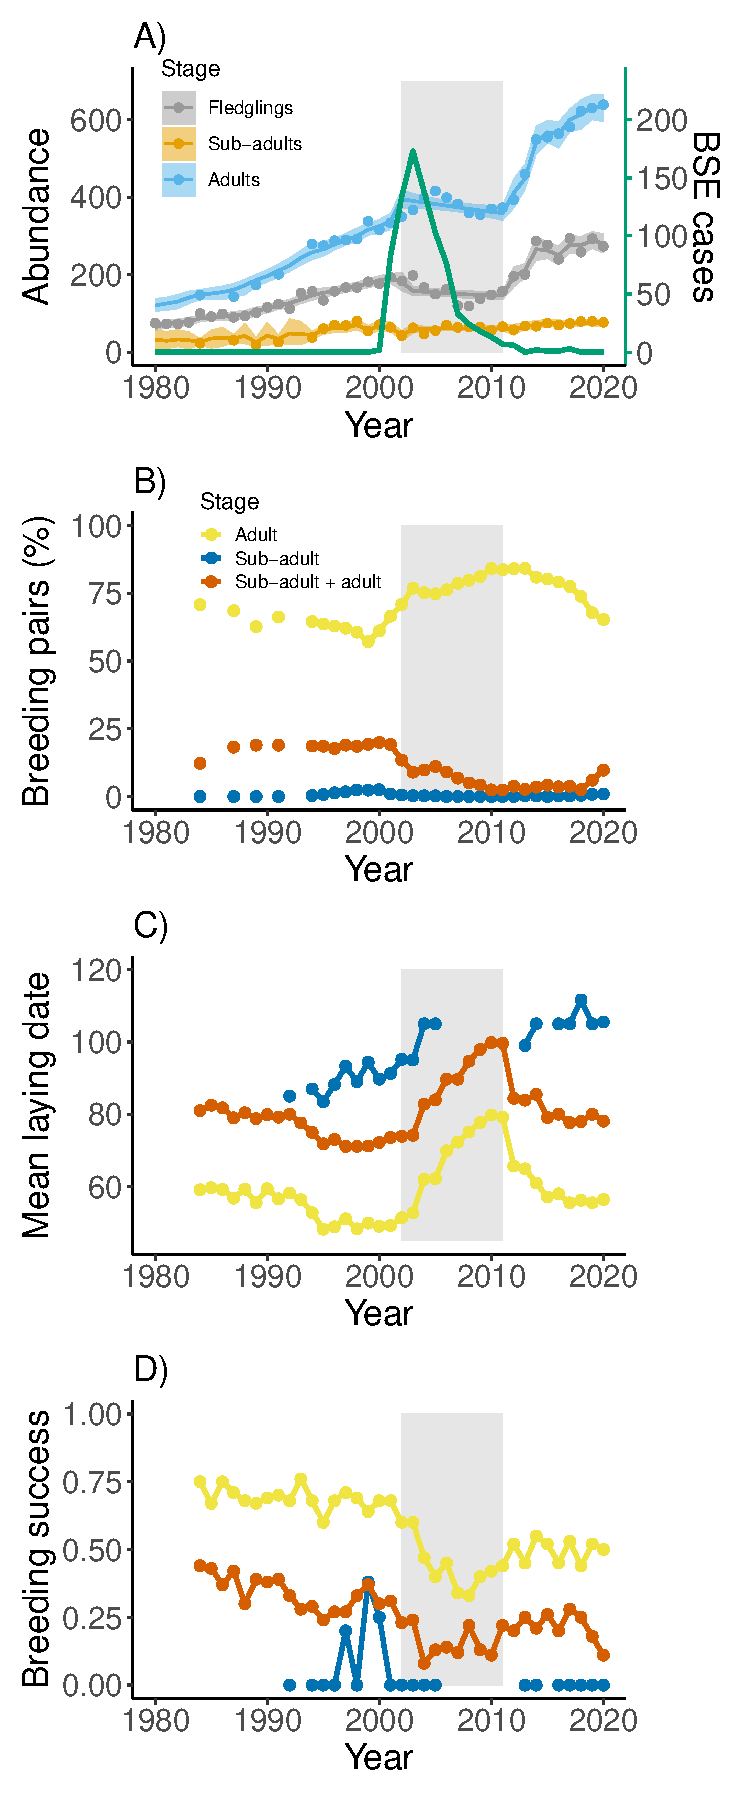
\includegraphics[width=8cm]{figs/Fig1.pdf}
	\end{center}
\end{figure}

\newpage
\begin{figure}[h!]
	\caption{}
	\label{Fig2}
	\begin{center}
		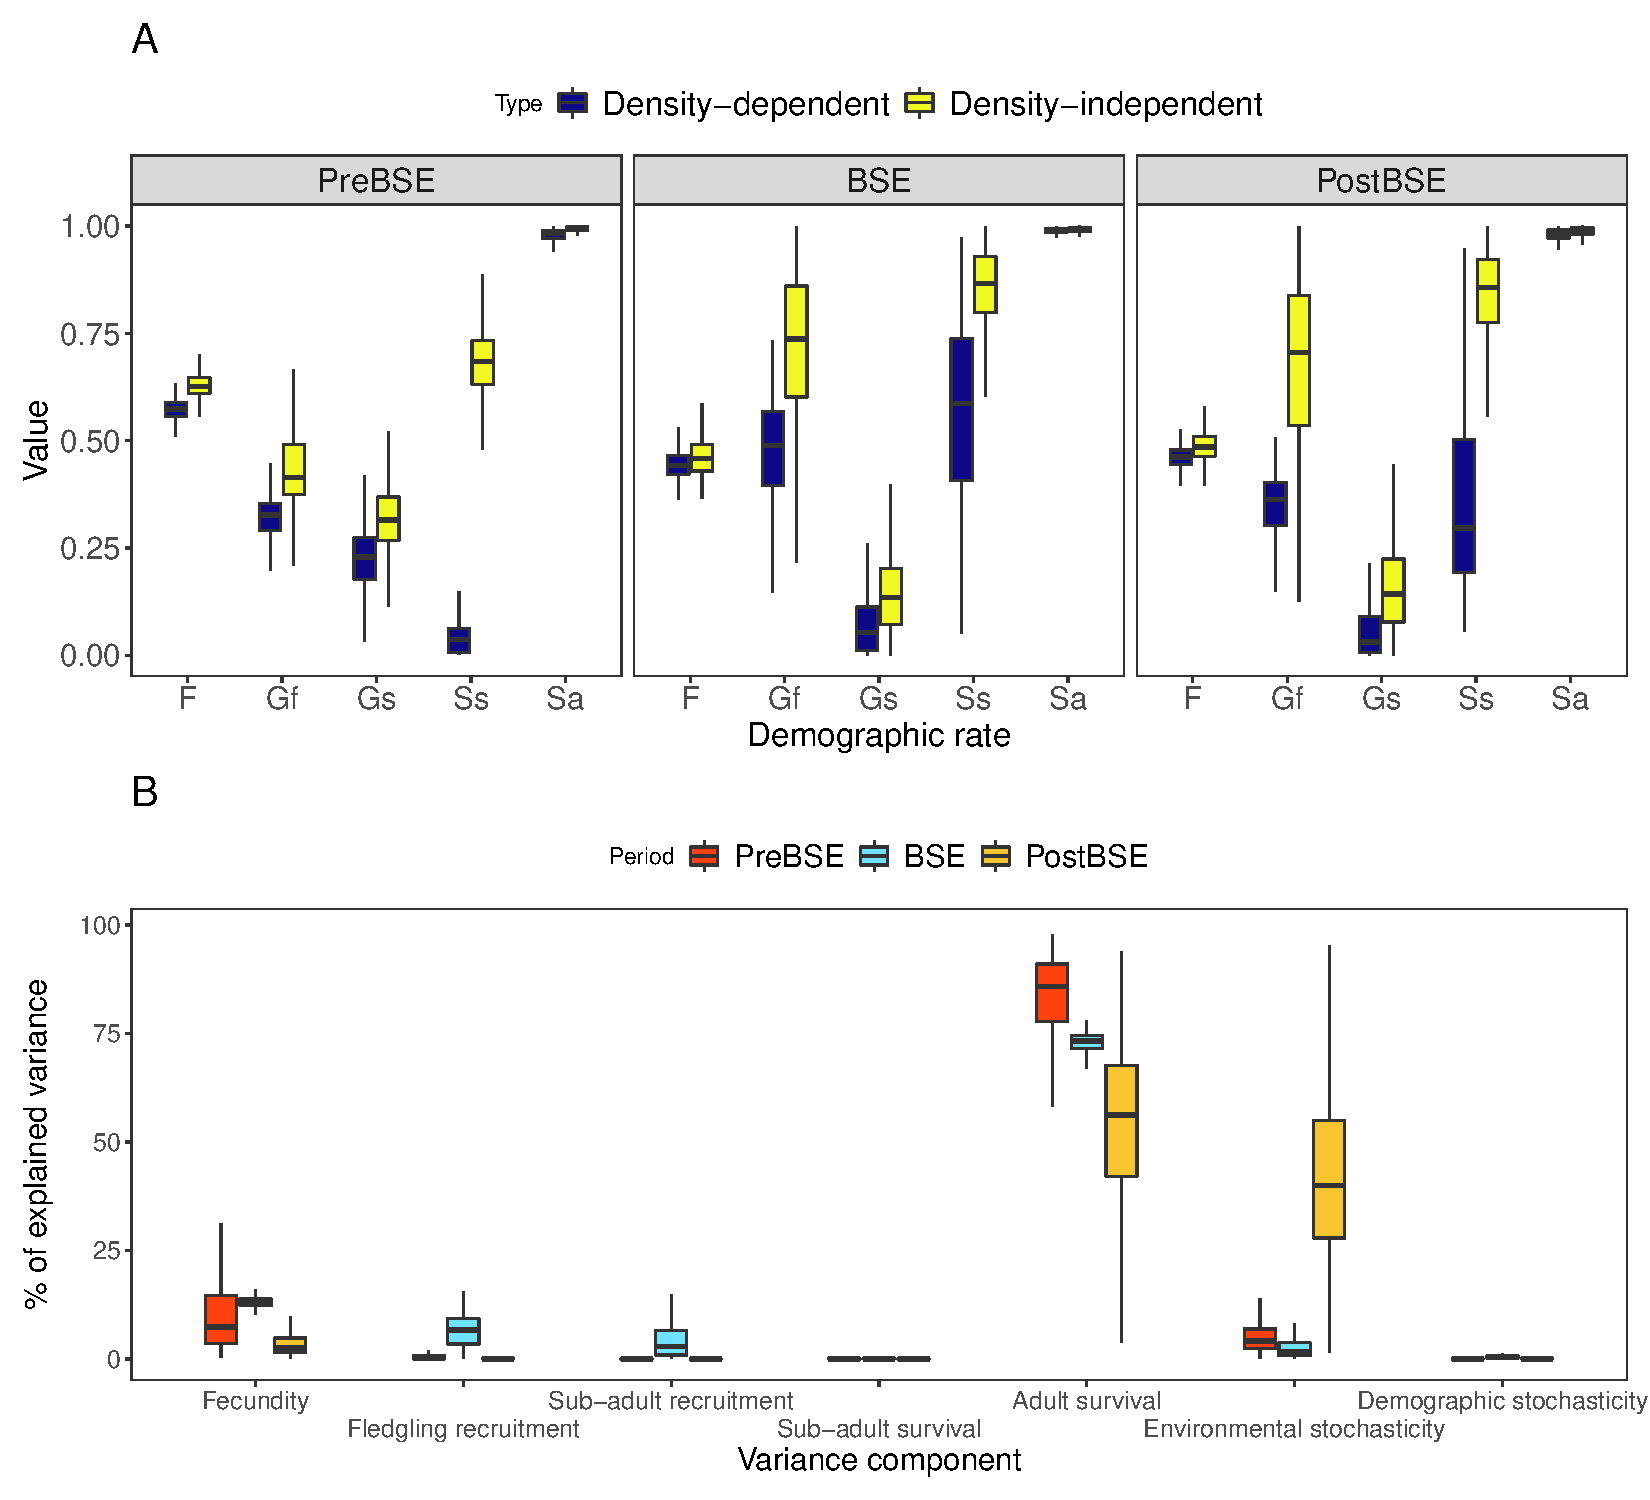
\includegraphics[width=15cm]{figs/Fig2.pdf}
	\end{center}
\end{figure}

\newpage
\begin{figure}[h!]
	\caption{}
	\label{Fig3}
	\begin{center}
		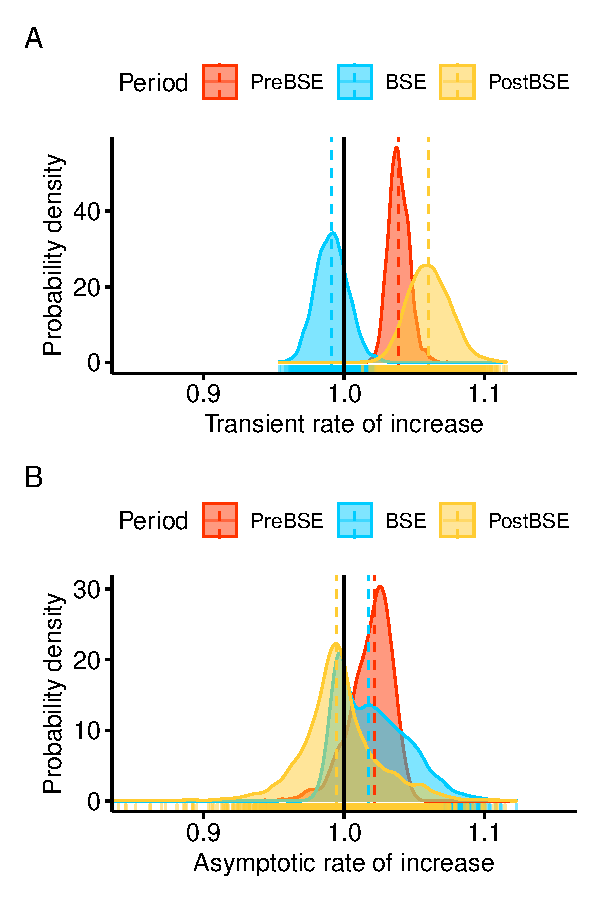
\includegraphics[width=8cm]{figs/Fig3.pdf}
	\end{center}
\end{figure}

\newpage
\begin{figure}[h!]
	\caption{}
	\label{Fig4}
	\begin{center}
		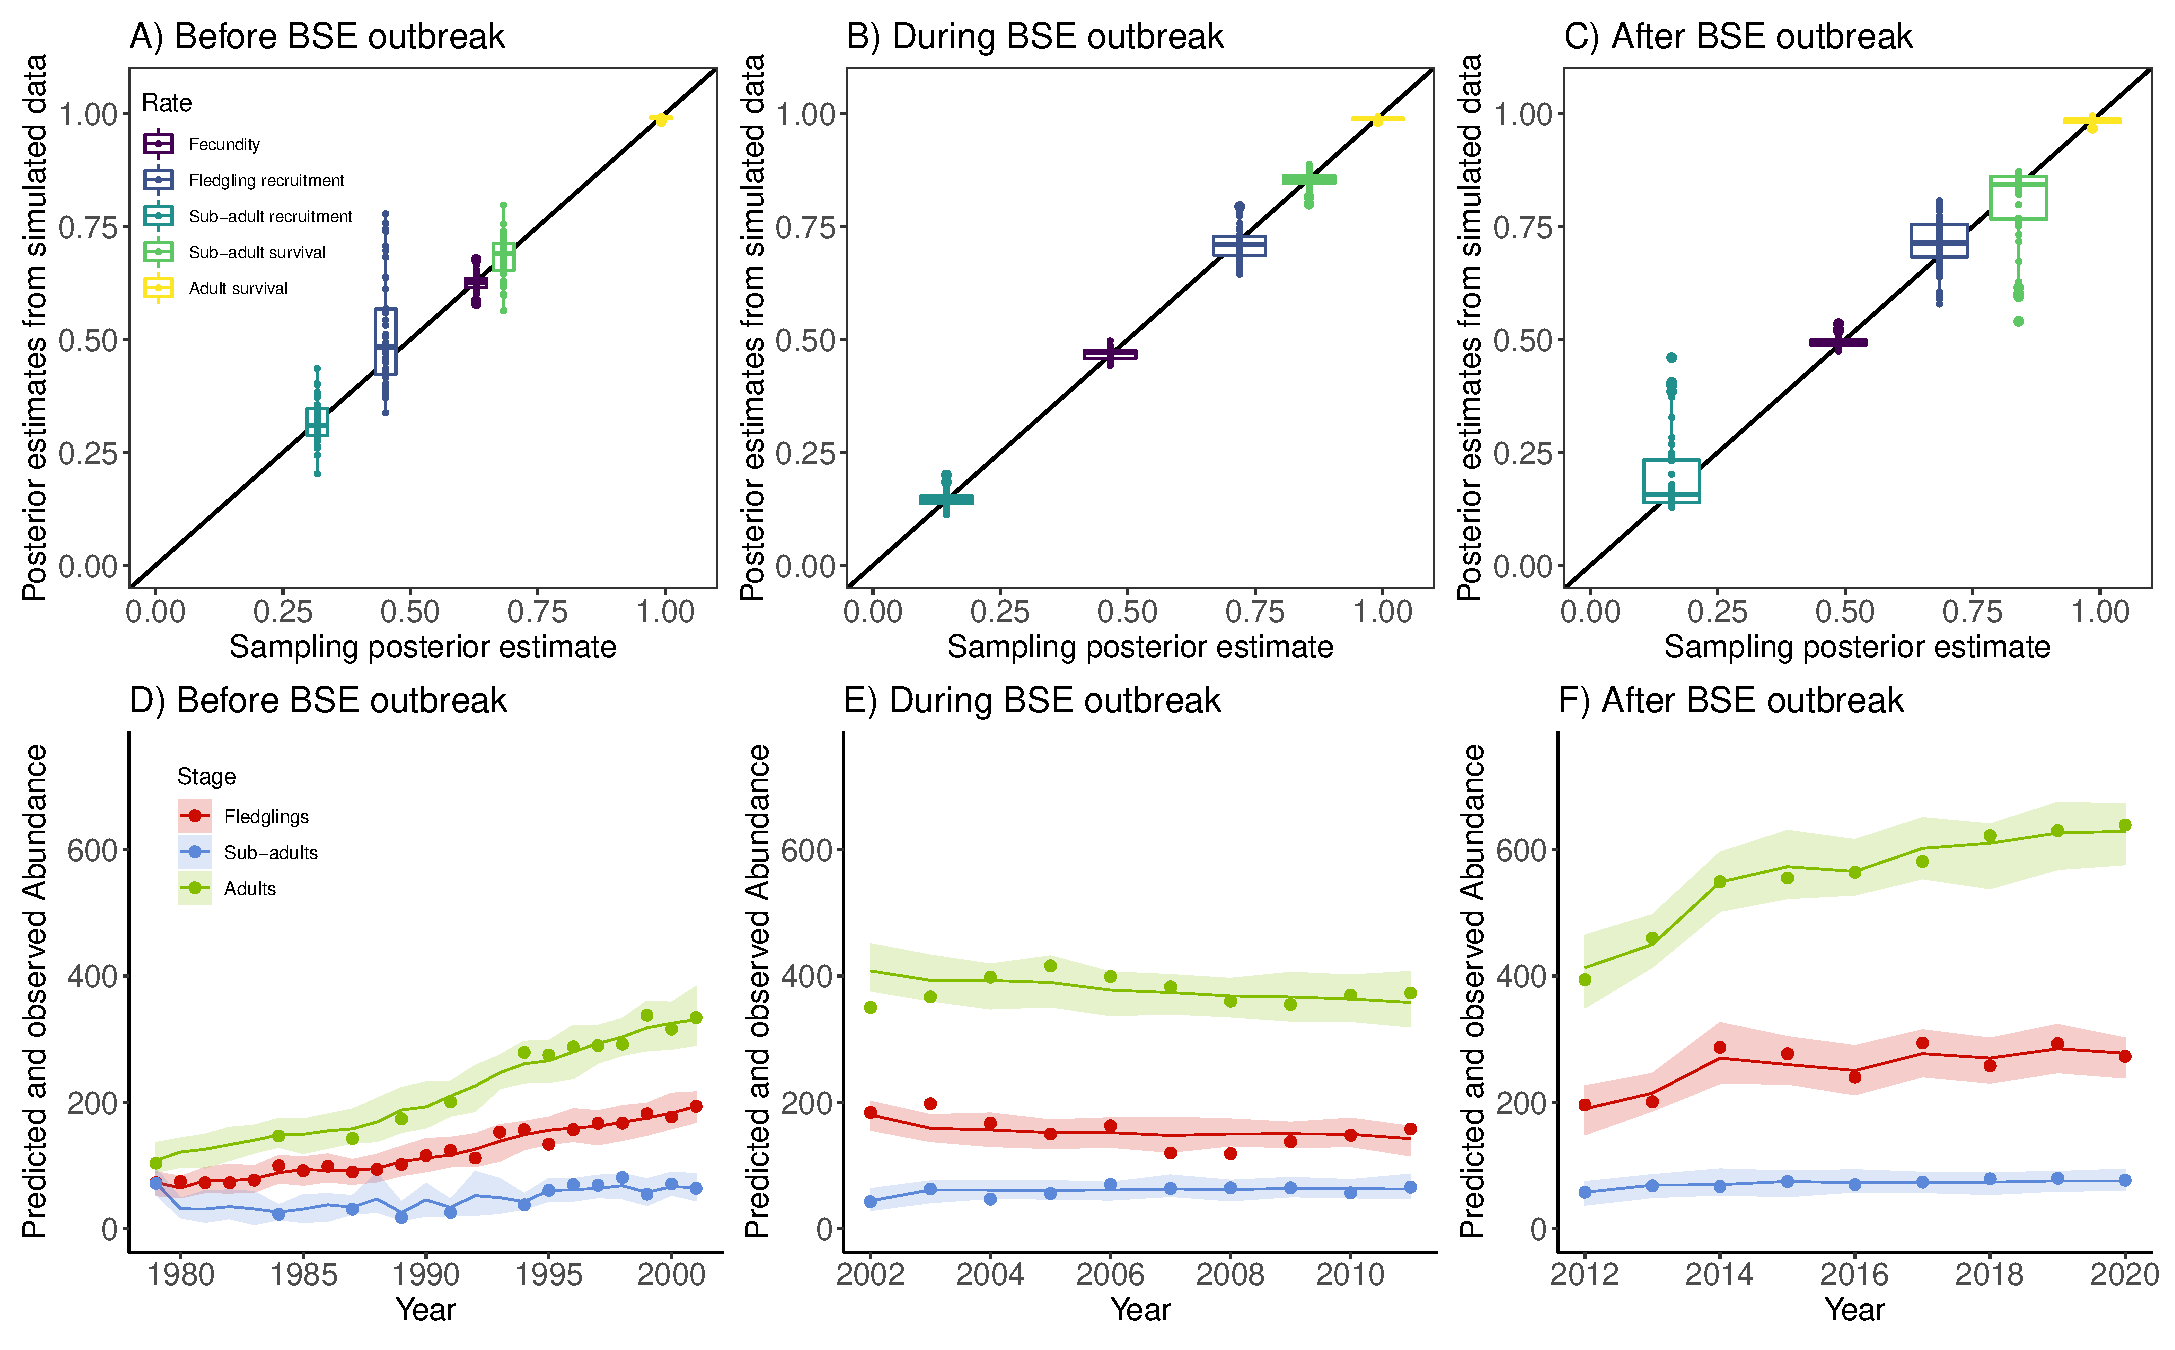
\includegraphics[width=16cm]{figs/Fig4.pdf}
	\end{center}
\end{figure}

%\includepdf[pages=1-5]{SupMat.pdf}

\end{document}